% Author: Jannes Bantje
% Modified: Lars Haalck lars.haalck@wwu.de
% please ask Lars Haalck first if you have any questions
\input{preamble.tex}

%path on which all content-related graphics for this document are stored
\graphicspath{ {./images/} }

%Informationen zur Arbeit
\newcommand{\printname}{Bastian Klein}
\newcommand{\printnumber}{XXX XXX}

\newcommand{\printtitle}{Leveraging MATLAB Simulink for Hexapod Robotics:\\Simulation, Control and Learning}
\newcommand{\printalttitle}{Nutzung von MATLAB Simulink in der Hexapod-Robotik: Simulation, Steuerung und Lernen}
\newcommand{\printcity}{Münster}
\newcommand{\printtype}{Bachelor's Thesis}
\newcommand{\printdegree}{Bachelor of Science}
\newcommand{\printsupervisor}{Prof. Dr. Malte Schilling \& Julius Adelt, M.Sc.}
\newcommand{\printfirstassessor}{Prof. Dr. Malte Schilling}
\newcommand{\printsecondassessor}{Prof. Dr. Paula Herber}
\newcommand{\printinstitute}{Computer Science Department}


\begin{document}

% set the pager numbering to big roman numbers for first few pages
\pagenumbering{roman}
\listoftodos

% titlepage does not need cleardoubleoddemptypage
\begin{titlepage}
	\input{chapter/title_page.tex}
\end{titlepage}

\begin{titlepage}
	\input{chapter/title_page2.tex}
\end{titlepage}

%\begin{titlepage}
%	%!TEX root = ../thesis.tex
\chapter{Exposé}
\label{ch:expose}



\section{Einleitung}
Der Einsatz von Simulationen spielt in der Erforschung und Entwicklung von Robotern eine zunehmend wichtige Rolle\parencite{afzal2020study}. 
Sie bieten eine kostengünstige und effiziente Methode, das Verhalten von Robotern schon vor der physischen Umsetzung untersuchen, analysieren und optimieren zu können\parencite{de2019analysis}. 
Auch eine Vielzahl von Unternehmen, welche auf dem Gebiet der Robotik tätig sind, nutzten die Technologie ausgiebig im Entwicklungsprozess ihrer Systeme, so beispielsweise Boston Dynamics\parencite{BostonDynamicsSimulation}, Tesla Inc.\parencite{TeslaAiDay2022} oder Kuka Robotics\parencite{KukaSim}.

Auf Grund ihrer hohen Beweglichkeit sowie Vielseitigkeit sind Hexapods in der Robotik von besonderen Interesse. 
Verglichen mit beräderten oder zweibeinigen Robotern können sie sich zuverlässiger auf unebenem Gelände bewegen und auch komplexe Hindernisse überwinden\parencite{barai2013smart, atifystructure}.
Die Simulation eines solchen Hexapods ermöglicht es sein Verhalten in verschiedensten simulierten Umgebungen zu beobachten und erproben.

\section{Problem}

Die Entwicklung von Robotern und ihren Bewegungsabläufen ist zeitaufwändig und mit hohen Kosten verbunden\parencite{ahmadian2005model}.
Wird die entwickelte Software direkt in der Realität getestet, so besteht die Gefahr der Beschädigung eines der oft wenigen und teuren Testexemplare.
Dies kann den Entwicklungsprozess verzögern und zusätzliche Kosten generieren.
Auch ist ein iterativer Optimierungsprozess, welcher ausschließlich in einer realen Umgebung stattfindet langsamer, als wenn dieser mit Hilfe von Simulationen unterstützt wird.
Die Steuerungssoftware muss für jede Anpassung neu auf die Hardware übertragen werden und Testaufbau sowie Roboter müssen manuell wieder in den Ausgangszustand versetzt werden.
Ebenfalls kann es schwierig sein fehlerhaftes Verhalten, welches beim Test mit einem realen System beobachtet wurde, zu reproduzieren, ohne die Möglichkeit einer exakten Wiederherstellung des Testaufbaus.

Natürlich ist es letztendlich wichtig, den entwickelten Controller auch in der echten Welt zu testen, damit sichergestellt werden kann, dass dieser auch unter den tatsächlichen physikalischen Begebenheiten zuverlässig funktioniert.
Die Vorteile welche eine Simulationsumgebung mit sich bringt sollten jedoch keinesfalls übersehen werden, da diese für Entwickler und Forscher ein mächtiges Werkzeug darstellen kann um vor der realen Erprobung erste Tests durchzuführen, Fehler aufzudecken und den Controller zu optimieren.
%Um die Erforschung von Controllern zu Bewegungssteuerung möglichst effektiv vorantreiben zu können ist es wichtig, leistungsstarke Simulationssoftware in den Entwicklungsprozess einzubeziehen.
%Es wird ein wesentlich  kleinschrittiger Prozess ermöglicht, da jede noch so kleine Änderung direkt und ohne großen Mehraufwand getestet werden kann.

%Da auf Grund von Materialkosten, Konstruktions- und Wartungsaufwand reale Roboter oft diejenige Komponente eines Projektes sind, welche beim Erproben der neu entwickelten Software der größte zeitliche "bottleneck" sind, stellt das direkte Erproben komplexer Aufgaben in der realen Welt(z.B. Navigation auf unebenem Gelände)  ein Risiko dar.

%Zur Entwicklung des Controllers und der Simulation desselben auf einem Hexapod-Modell wird in dieser Arbeit das MATLAB Tool Simulink in Verbindung mit der Simulation-Toolbox SimScape verwendet werden.
%Simulink ist eine weit verbreitete Software zur Entwicklung und Simulation von komplexen dynamischen Systemen.
%Durch die Popularität der Software ist mit der Zeit eine Vielzahl von domänenspezifischen Bibliotheken(Toolboxes) entstanden, welche die einfache Modellierung verschiedenster Modelle ermöglichen.
%Der block-basierte Ansatz von Simulink ist dabei besonders hervorzuheben, da es dieser ermöglicht sehr modulare Systeme zu erzeugen, wodurch bei Anpassungen nur einzelne Subsysteme ausgetauscht werden, anstatt Änderungen am gesamten Modell vornehmen zu müssen.

\section{Ziel}
Das von uns im Rahmen dieser Bachelorarbeit angestrebte Ziel ist es, die Möglichkeiten von MATLAB Simulink zur Modellierung und Simulation komplexer dynamischer Systeme zu nutzen, um ein Modell eines Hexapod-Roboters sowie dessen Steuerung zu entwickeln.

Das Modell muss die kinematischen Eigenschaften des Roboters und der Umgebung in welcher er sich bewegt berücksichtigen.
Es soll eine realistische Simulation des Roboterverhaltens ermöglichen und dabei Informationen bezüglich der Positionierung des Modells bereitstellen.
Diese Daten sind entscheidend für die Steuerung des Roboters und müssen für den Controller jederzeit zur Verfügung stehen.
Der Bewegungscontroller des Hexapods sollte in der Lage sein, den Roboter zuverlässig und präzise zu steuern.
Dies beinhaltet die Bewegung des einzelnen Beins, die Koordination der Beine untereinander sowie das Gleichgewicht des Gesamtsystems aufrecht zu erhalten.
Die entwickelte Lösung soll den Roboter in verschiedenen Gangarten geradlinig in der Simulationsumgebung bewegen und auch kleine Hindernisse überwinden können, ohne dass das System aus dem Gleichgewicht gebracht wird.
Dabei darf die Steuerung nur auf vom Modell bereitgestellte Daten zugreifen, wie dies auch bei einem realen Roboter mittels Sensoren der Fall wäre.
Es sollte zusätzlich möglich sein, Module des Bewegungscontrollers anzupassen oder Eigenschaften des Modells zu ändern, ohne den gesamten Roboter neu konfigurieren zu müssen.
Nachdem ein robustes Modell und ein zuverlässiger Controller entwickelt wurden liegt der Fokus darauf, es dem Roboter mit Hilfe von maschinellem Lernen zu ermöglichen, die Koordination der Beine selbständig zu erlernen.
Es wäre besonders interessant festzustellen, ob schon bekannte Gangarten erkennbar werden oder ganz neue Formen der Bewegung entstehen.


\section{Ziel}
Das angestrebte Ziel dieser Bachelorarbeit ist es, einen Hexapod-Roboter und dessen Steuerung innerhalb der MATLAB Simulink Umgebung zu entwickeln.
Konkret soll dies die Modellierung des physischen Modells mit Hilfe von SimScape, den Aufbau eines Controllers für die Bewegungssteuerung des Roboters sowie das Erlernen der Koordination der Beine untereinander mittels Reinforcement Learning beinhalten.

\begin{enumerate}
	
	
	\item \textbf{Selbstständiges Erlernen der Beinkoordination:} Durch Interaktion mit der Simulationsumgebung soll das Modell selbstständig die Koordination der 6 Beine erlernen, die Beinbewegung selbst bleibe dabei vorgegeben.
	Modelliert werden soll der Lernprozess mit Hilfe der Reinforcement Learning Toolbox von Simulink.
	
\end{enumerate}

\section{Lösungsansatz}
Zu Beginn der Arbeit wird ein detailliertes, physikalisch korrektes Modell des Hexapods mithilfe der Simulink-Toolbox Simscape entwickelt, als Vorlage dient hier der \emph{PhantomX}-Hexapod von \emph{Trossen Robotics}.
Jedes der 6 Beine besteht aus 3 Gelenken mit je einem Aktuator, eine Architektur welche weit verbreitet ist und sich bewährt hat.
Das Modell sollte möglichst gut parametrisiert werden, damit Eigenschaften wie Gewicht, Reibungskoeffizienten, Drehmomente, etc. der einzelnen Komponenten auch im nach hinein noch einfach angepasst werden können.
Jeder der Aktuatoren muss einzeln ansprechbar sein und die Gelenke müssen Sensordaten bezüglich Position (und Beschleunigung) liefern.
Diese Daten informieren den im nächsten Schritt zu implementierenden Controller über die Lage (und Dynamik) des Roboters.
Neben dem eigentlichen Modell des Hexapods wird zusätzlich noch eine einfache Testumgebung erbaut, in welcher das Robotermodell im weiteren Entwicklungsprozess ausgiebig getestet werden kann.

Nachdem die Entwicklung des SimScape-Modells abgeschlossen ist, wird mit der Implementierung einer kontrollierten Steuerung des Roboters in Simulink begonnen.
Der Fokus liegt dabei zunächst auf der Beschreibung des Bewegungsablaufs eines einzelnen Beins.
Sobald dieser Ablauf, bestehend aus Schwung- und Standphase, zuverlässig funktioniert, wird er auf alle 6 Beine ausgeweitet.
Hierbei spielt die Koordination der Beine eine entscheidende Rolle, unabhängig davon, ob diese zentral oder verteilt ausgelegt wird.
Grundlegend ist es natürlich auch, dass der Roboter das Gleichgewicht hält und robust gegenüber Störungen im Bewegungsablauf ist.
Um das SimScape-Modell ausgiebig zu testen, ist es möglich, mehrere verschiedene Gangarten wie den Tripod-, Tetrapod- und Wave-Gait abzubilden.
%evt. könnte auch eine dezentrale Architektur wie z.B. die von Schilling et al. abgebildet werden (?).

Basierend auf den Vorarbeiten zur Modellierung und den verschiedenen Gangarten soll anschließend die Koordination der Beine mithilfe eines Reinforcement Learning-Modells selbst erlernt werden.
Dieser Lernprozess wird ebenfalls innerhalb der Simulink-Umgebung durch die RL-Toolbox realisiert.
Im Gegensatz zu den bisher erzeugten Gangarten wird hier nicht vorgegeben werden, welche Beine ihren Bewegung zu welchem Zeitpunkt ausführen sollen.
Der Bewegungsablauf eines einzelnen Beins bleibt vorgegeben, während die Koordination untereinander durch Interaktion des Modells mit der Umgebung erlernt werden soll. 
Diese Herangehensweise ermöglicht es die Komplexität der zu erlernenden Fähigkeiten zunächst zu reduzieren, lässt aber gleichzeitig die Möglichkeit offen, im weiteren Verlauf zusätzliche Elemente in den Lernprozess einzubeziehen.


\section{Verwandte Arbeiten}
\textbf{TODO: Ausformulieren !}
\begin{enumerate}

\item SMART-HexBot: a Simulation, Modeling, Analysis and
Research Tool for Hexapod Robot in Virtual Reality and
Simulink

\item Design, Simulation, and Control of a Hexapod Robot in
Simscape Multibody

\item Dynamic Modeling and Control of the Hexapod Robot Using Matlab SimMechanics

\end{enumerate}


\section{Zeitplan}
\begin{enumerate}
	\item Erstellen des "physischen" Hexapod-Modells in Simulink/Simscape + Testumgebung:
	\begin{enumerate}[label*=\arabic*.]
		\item Import eines 3D-Modells in die Simulink-Umgebung
		\item Konfigurieren eines "Inverse Kinematics Solvers" basierend auf der .urdf-Datei des 3D-Modells
		\item Definieren der Parameter des Roboters(Drehmomente der Motoren, Reibungskoeffizienten zwischen Beinen und Boden, max. Winkel, etc.)
		\item Erbauen einer einfachen Testumgebung
	\end{enumerate}
	\textbf{Geschätzte Dauer:} 2-3 Wochen
	
	\item Entwicklung des Bewegungscontrollers
	\begin{enumerate}[label*=\arabic*.]
		\item Bewegungsablauf eines einzelnen Beins
		\item Implementierung der Gangarten(Wave-, Tripod, etc.)	
		\item Erprobung und Optimierung der Bewegungen des Hexapods innerhalb der Simulationsumgebung
	\end{enumerate}
	\textbf{Geschätzte Dauer:} 3-4 Wochen
	
	\item Erlernen der Beinkoordination
	\begin{enumerate}[label*=\arabic*.]
		\item Aufstellen des Reinforcement Learning-Modells
		\item Beobachten des Lernprozesses, ggf. Anpassungen vornehmen
	\end{enumerate}
	\textbf{Geschätzte Dauer:} 4 Wochen
	

\end{enumerate}


Abschluss der Arbeit hoffentlich (Ende) September.
%\end{titlepage}

%!TEX root = ../thesis.tex
\begin{abstract}
\section*{Abstract}
In recent years, driven by their unique capabilities, the research on hexapod robots has gained significant traction.
These systems, able to navigate challenging terrain and overcome complex obstacles, hold the promise to advancements in various domains.
While hexpods possess significant potential, real-world applications remain rare, and substantial research is still required to further enhance the current systems. Given the intricacies of hexapod robots as complex mechanical machines, the utilization of simulation software offers numerous advantages.
With this thesis we aim to add to the array of existing simulators by providing a comprehensive, modular and physically accurate model of a hexapod robot using the MATLAB Simulink environment.
The model we develop aims to lay the foundation for future research to build on.
During the course of our work we continuously test the model in numerous simulations, ensuring the functionality of each module and the final product as a whole.
For this purpose, we conceive a simple locomotion controller, enabling omnidirectional locomotion of the hexapod in several different, static gait patterns.
Furthermore, we develop the capabilities to apply Reinforcement Learning to problem of autonomously learning efficient leg coordination strategies, highlighting the versatility of the MATLAB-platform and providing impulses for future research to expand upon these efforts. 

\end{abstract}

%\cleardoubleoddemptypage

\tableofcontents
%\cleardoubleoddemptypage

% set the page numbering back to arabic
\pagenumbering{arabic}
\setcounter{page}{1}

\begin{titlepage}
	%!TEX root = ../thesis.tex
\chapter{Introduction}
\label{ch:introduction}


%\textbf{INTRODUCTION:}
Simulations play an increasingly important role in robotics research and development \parencite{afzal2020study}. 
They offer a cost-effective and efficient means to investigate, analyze and optimize the behavior of robots even before they are physically implemented \parencite{de2019analysis}. 
Notably, various companies involved in the field of robotics use simulation technology extensively in the development process of their systems, such as Boston Dynamics \parencite{BostonDynamicsSimulation}, Tesla Inc. \parencite{TeslaAiDay2022} or Kuka Robotics \parencite{KukaSim}.
Due to their high degree of mobility and versatility, hexapods are of particular interest in robotics. 
Compared to wheeled or bipedal architectures, the presence of six legs enables these robots to more easily overcome challenging terrain and complex obstacles \parencite{barai2013smart, atifystructure}, making them particularly interesting for navigating landscapes otherwise inaccessible to humans or other types of robotic systems.

\textbf{PROBLEM:}
\todo{Reads to much like defining the goals I want to achieve}
The process of developing software for these hexapods is a challenging and by no means trivial task.
While maintaining balance for instance, is evidently easier for this architecture than for the above mentioned bipedal robots, coordinating the many legs during movement poses a major challenge \parencite{azayev2020blind,schilling2013walknet}.
When trying to break down the complex dynamics of such a system, the creation of a virtual model can present 
numerous advantages.

Trying to base the complete software verification process solely on the real robotic hardware can pose multiple problems.
Firstly, there is a heavy reliance on the hardware.
Without a functioning robot, the development process comes to a standstill.
As physical robots are costly, the actual number of robots available is often low if not singular.
If the software is not functioning well, the robot can fall or otherwise damage itself.
This can lead to high repair times and costs, both of which are undesirably.
Another problem with solely testing on hardware is the missing complete reproducibility a simulation can offer.
If the software contains edge cases which only occur in very specific configurations, these are extremely hard to reproduce in the real world because no test setup can be exactly the same.
A simulation can provide this reproducibility, given the same inputs it will always produce the same outputs.

In order to support and accelerate our research on hexapod robots, we aim to capitalize on these benefits.
We seek an environment which offers a wide range of tools to enhance our understanding of the robots behavior as well as enables us to more quickly verify and optimize new ideas.
In our search for an adequate solution, we found a variety of robot simulation platforms, such as Gazebo, V-REP or Webots. 
Each of these simulators has its own strengths and features that researchers have utilized to explore different aspects of robotics \parencite{de2019analysis}.
Besides these tools explicitly developed for simulating robots, there are other modeling and simulation environments which have a wider fiend of use.
One example of these is \textit{MATLAB Simulink\textsuperscript{\textregistered}}, a graphical programming environment used for modeling, simulation and analysis of complex, dynamic systems \parencite{Simulink}.
In recent years, several scientific papers have been published dealing with the simulation of a hexapod in Simulink(see e.g. \cite{tanaka2019development, barai2013smart, atify2019propelling}).
However, to our knowledge, there is currently no publicly available, up-to-date Simulink-based hexapod model on which further research could build on.
%Simulink's diagram-like interface and extensive library of "toolboxes" facilitate the creation of modular and well-organized systems, which can also be immediately simulated.
Considering the widespread use of Simulink in both research and industry along with its extensive libraries addressing various domains, we have chosen it as our preferred platform.
%In our opinion, the MATLAB Simulink modeling and simulation environment from the MathWorks company is particularly interesting for implementing such a model.
%Due to its diagram-like development interface based on functional blocks and a large number of so-called "toolboxes" from a wide variety of application areas, Simulink enables the generation of modular and clearly arranged systems, which can be simulated immediately.



%Auf Grund ihrer hohen Beweglichkeit und Vielseitigkeit sind Hexapods in der Robotik von besonderen Interesse. 
%Verglichen mit beräderten oder zweibeinigen Robotern können sie sich zuverlässiger auf unebenem Gelände bewegen und auch komplexe Hindernisse überwinden \parencite{barai2013smart, atifystructure}.
%Die Programmierung eines Bewegungscontrollers für solch einen Hexapod-Roboter ist eine anspruchsvolle, keinenfalls triviale Aufgabe.
%Obwohl das Aufrechterhalten der Balance bei einem Roboter mit 6 Beinen im Vergleich zu beispielsweise humanoiden Zweibeinern offensichtlich einfacher ist, stellt die Koordination der vielen Beine während der Fortbewegung eine große Herausforderung dar \parencite{azayev2020blind,schilling2013walknet}.
%Die Erzeugung eines virtuellen Modells kann hierbei viele Vorteile mit sich bringen.
%Es ermöglicht Designkonzepte zu testen, die Bewegung des Roboters zu analysieren und die Leistungsfähigkeit des Systems schon vor der physischen Umsetzung zu beurteilen \parencite{de2019analysis}.

%Besonders interessant für die Umsetzung eines solchen Modells ist unserer Meinung nach die Modellierungs- und Simulationsumgebung MATLAB Simulink des Unternehmens MathWorks.
%Durch die auf funktionalen Blöcken basierende, diagrammartige Entwicklungsoberfläche und eine Vielzahl sog. "Toolboxes" aus unterschiedlichsten Anwendungsgebieten ermöglicht Simulink die Erzeugung modularer und übersichtlicher Systeme, welche sofort simuliert werden können.
%In den letzten Jahren wurden mehrere wissenschaftliche Arbeiten veröffentlicht, die sich mit der Simulation eines Hexapods in Simulink beschäftigen(siehe z.B. \cite{tanaka2019development, barai2013smart, atify2019propelling}), sodass sich schließen lässt, dass die Vorteile der simulationsgestützten Entwicklung durchaus wahrgenommen und genutzt werden.
%Jedoch gibt es unseren Wissens nach derzeit kein öffentlich verfügbares, modernes Simulink-Modell auf dem weitere Forschung aufbauen könnte.

%Wir wollen uns in dieser Bachelorarbeit deshalb dem Problem der Entwicklung eines solchen Modells mit Hilfe von Simulink widmen.



%Um die Erforschung von Controllern zu Bewegungssteuerung möglichst effektiv vorantreiben zu können ist es wichtig, leistungsstarke Simulationssoftware in den Entwicklungsprozess einzubeziehen.
%Es wird ein wesentlich  kleinschrittiger Prozess ermöglicht, da jede noch so kleine Änderung direkt und ohne großen Mehraufwand getestet werden kann.

%Da auf Grund von Materialkosten, Konstruktions- und Wartungsaufwand reale Roboter oft diejenige Komponente eines Projektes sind, welche beim Erproben der neu entwickelten Software der größte zeitliche "bottleneck" sind, stellt das direkte Erproben komplexer Aufgaben in der realen Welt(z.B. Navigation auf unebenem Gelände)  ein Risiko dar.

%Zur Entwicklung des Controllers und der Simulation desselben auf einem Hexapod-Modell wird in dieser Arbeit das MATLAB Tool Simulink in Verbindung mit der Simulation-Toolbox SimScape verwendet werden.
%Simulink ist eine weit verbreitete Software zur Entwicklung und Simulation von komplexen dynamischen Systemen.
%Durch die Popularität der Software ist mit der Zeit eine Vielzahl von domänenspezifischen Bibliotheken(Toolboxes) entstanden, welche die einfache Modellierung verschiedenster Modelle ermöglichen.
%Der block-basierte Ansatz von Simulink ist dabei besonders hervorzuheben, da es dieser ermöglicht sehr modulare Systeme zu erzeugen, wodurch bei Anpassungen nur einzelne Subsysteme ausgetauscht werden, anstatt Änderungen am gesamten Modell vornehmen zu müssen.


\textbf{OBJECTIVE:}
Our main goal for this thesis is to develop a comprehensive virtual model of a hexapod robot using the MATLAB Simulink\textsuperscript{\textregistered} environment.
The model we develop will serve as a foundation for future research to build on.
Facilitating flexible and easy expansions to the model, a high level of modularity is required, allowing for the integration or replacement of modules without the need to reconfigure the whole system.
It is essential that the created model interacts in a physically correct way with the simulated surrounding, giving us a testbed as close to reality as possible.
Additionally, accessible means to observe and analyze the robots behavior are provided.
This includes the capability to extract and evaluate data from the simulation, enabling us to gain valuable insights into the systems performance.
Furthermore, the integration with the MATLAB software framework opens up possibilities to incorporate learning algorithms into the model.
Utilizing these, we will be able to optimize various aspects of the robotic system. 
This includes fine-tuning of control algorithms using Reinforcement Learning, enabling the robot to autonomously learn efficient leg movements and develop coordination strategies.
The model will also provide a basis for testing more advanced learning algorithms, such as vision-based path planing and terrain-navigation.

To validate the developed model, we implement a motion controller which allows the robot to navigate within the virtual environment in straight lines. This also includes the application of Reinforcement Learning, enabling the robot to learn "interlimb" coordination from the ground up.
To prove its functionality, the controller has to be able to steer the robot smoothly and reliably while maintaining its overall balance.
It also needs to show the capability of performing different gait patters as well as traversing slightly uneven terrain.
\todo{Uneven terrain not planned to be included}


%\section{Ziel}
%Das von uns im Rahmen dieser Bachelorarbeit angestrebte Ziel ist es, die Möglichkeiten von MATLAB Simulink zur Modellierung und Simulation komplexer dynamischer Systeme zu nutzen, um ein Modell eines Hexapod-Roboters sowie dessen Steuerung zu entwickeln.
%Wir wollen mit den Ergebnissen dieser Arbeit die Vorteile eines durch Simulink gestützten Entwicklungsprozesses hervorheben und Impulse für eine ausgiebigere Nutzung derartiger Software setzen.

%Das Modell muss die kinematischen Eigenschaften des Roboters und der Umgebung in welcher er sich bewegt berücksichtigen.
%Es soll eine realistische Simulation des Roboterverhaltens ermöglichen und dabei Informationen bezüglich der Positionierung des Modells bereitstellen.
%Diese Daten sind entscheidend für die Steuerung des Roboters und müssen für den Controller jederzeit zur Verfügung stehen.
%Der Bewegungscontroller des Hexapods sollte in der Lage sein, den Roboter zuverlässig und präzise zu steuern.
%Dies beinhaltet die Bewegung des einzelnen Beins, die Koordination der Beine untereinander sowie die Gleichgewichtserhaltung des Gesamtsystems.
%Die entwickelte Lösung soll den Roboter in verschiedenen Gangarten geradlinig in der Simulationsumgebung bewegen und auch kleine Hindernisse überwinden können, ohne dass das System aus dem Gleichgewicht gebracht wird.
%Dabei darf die Steuerung nur auf vom Modell bereitgestellte Daten zugreifen, wie dies auch bei einem realen Roboter mittels Sensoren der Fall wäre.
%Es sollte außerdem möglich sein, Module des Bewegungscontrollers anpassen zu können oder Eigenschaften des Modells abzuändern, ohne das gesamte System neu konfigurieren zu müssen.
%Nachdem ein robustes Modell und ein zuverlässiger Controller entwickelt wurden liegt der Fokus darauf, es dem Roboter mit Hilfe von maschinellem Lernen zu ermöglichen, die Koordination der Beine selbständig zu erlernen.
%Es wäre besonders interessant festzustellen, ob schon bekannte Gangarten erkennbar werden oder ganz neue Formen der Bewegung entstehen.


\todo{Check for passive formulations --> change to active}
\todo{Rewrite without chronological order; begin with key ideas}
\todo{Include Sanandos model}
\textbf{PROPOSED SOLUTION:}

%THIS SECTION WAS TRNSFERED FROM "OBJECTIVE"

%The model must take into account the kinematic properties of the robot and the environment in which it moves.
%It should allow a realistic simulation of the robot's behavior while providing information regarding the positioning of the model.
%This data is critical for controlling the robot and must be available to the controller at all times.
%The motion controller of the Hexapod should be able to control the robot reliably and precisely.
%This includes the movement of the individual leg, the coordination of the legs with each other, and the balance maintenance of the overall system.
%The developed solution should be able to move the robot in different gaits in a straight line in the simulation environment and also overcome small obstacles without unbalancing the system.
%In doing so, the controller must only access data provided by the model, as would be the case with a real robot using sensors.
%It should also be possible to adjust modules of the motion controller or change properties of the model without having to reconfigure the entire system.
%After a robust model and a reliable controller have been developed, the focus is on using machine learning to enable the robot to learn leg coordination on its own.
%It would be particularly interesting to determine if already familiar gaits become recognizable or if entirely new forms of movement emerge.

The majority of work done for this thesis is based on and supported by the \textit{MATLAB\textsuperscript{\textregistered}} software framework and the MATLAB-based \textit{Simulink\textsuperscript{\textregistered}} environment, both developed by the company \textit{MathWorks\textsuperscript{\textregistered}}.
Simulink provides a graphical block diagramming tool, which enables a very modular and visually clear development process.
Through a multitude of so-called "toolboxes", complex dynamic models from a wide variety of application areas can be created.

Initially, we construct a detailed, physically correct model of the hexapod using Simulink's Toolbox \textit{Simscape\textsuperscript{\texttrademark}}, taking the \emph{PhantomX} hexapod developed by \emph{Trossen Robotics} as a template.
The model is parameterized as well as possible, so that properties like weight, friction coefficients or max. applied torques of the individual components can be easily adjusted later on.
Each of the models actuators is individually addressable and provides sensor data regarding position (and acceleration).
Additionally, a simple test environment is constructed to extensively test the robot model during the further development process.

The subsequent step focuses on the implementation of a motion controller enabling the hexapod to walk.
Initially, the attention lies only on defining the motion of a single leg.
When this sequence, consisting of "swing" and "stance" phase, works reliably, it is extended to all six legs.
Here, coordinating the legs in such a way that an efficient walking motion emerges, is of special importance.
It is also fundamental of course, that the robot maintains balance and is robust in the face of disturbances throughout the entire movement sequence.
In order to extensively test the Simscape model, we implement several different gaits such as the tripod, tetrapod and wave gait.
%evt. a decentralized architecture such as that of Schilling et al. could also be represented (?).

Based on the preliminary work done on the model and different gaits, we use a reinforcement learning(RL) approach to learn the coordination of the legs.
This learning process is also realized within the Simulink environment utilizing the RL toolbox.
In contrast to the gaits generated so far, only the motion sequence of the individual leg remains fixed, while the coordination among them is learned by interaction of the model with its environment. 
This approach of keeping the individual legs motion predefined, makes it possible to initially reduce the complexity of the skills to be learned, but at the same time leaves open the possibility of including additional elements in the learning process as it progresses.

%\section{Lösungsansatz}
%Die Grundlage der Arbeit liefert die in der Forschung und Industrie weit verbreite Software \textit{MATLAB\textregistered} und die enthaltene \textit{Simulink}\textregistered-Umgebung des Unternehmens \textit{MathWorks}.
%Simulink bietet eine auf funktionalen Blöcken basierende Modellierungsmethode, welche einen sehr modularen und visuell übersichtlichen Entwicklungsprozess ermöglicht.
%Durch eine Vielzahl von sogenannten "Toolboxes" können Modelle aus den verschiedensten Anwendungsgebieten erschaffen werden.
%
%Zu Beginn der Arbeit wird ein detailliertes, physikalisch korrektes Modell des Hexapods mithilfe der Simulink-Toolbox Simscape entwickelt, als Vorlage dient hier der \emph{PhantomX}-Hexapod von \emph{Trossen Robotics}.
%Jedes der 6 Beine besteht aus 3 Gelenken mit je einem Aktuator, eine Architektur welche weit verbreitet ist und sich bewährt hat.
%Das Modell sollte möglichst gut parametrisiert werden, damit Eigenschaften wie Gewicht, Reibungskoeffizienten, Drehmomente, etc. der einzelnen Komponenten auch im nach hinein noch einfach angepasst werden können.
%Jeder der Aktuatoren muss einzeln ansprechbar sein und die Gelenke müssen Sensordaten bezüglich ihrer Position (und Beschleunigung) liefern.
%Diese Daten informieren den im nächsten Schritt zu implementierenden Controller über die Lage (und Dynamik) des Roboters.
%Neben dem eigentlichen Modell des Hexapods wird zusätzlich noch eine einfache Testumgebung erbaut, in welcher das Robotermodell im weiteren Entwicklungsprozess ausgiebig getestet werden kann.
%
%Nachdem die Entwicklung des SimScape-Modells abgeschlossen ist, wird mit der Implementierung einer kontrollierten Steuerung des Roboters in Simulink begonnen.
%Der Fokus liegt dabei zunächst auf der Beschreibung des Bewegungsablaufs eines einzelnen Beins.
%Sobald dieser Ablauf, bestehend aus Schwung- und Standphase, zuverlässig funktioniert, wird er auf alle 6 Beine ausgeweitet.
%Hierbei spielt die Koordination der Beine eine entscheidende Rolle, unabhängig davon, ob diese zentral oder verteilt ausgelegt wird.
%Grundlegend ist es natürlich auch, dass der Roboter das Gleichgewicht hält und robust gegenüber Störungen im Bewegungsablauf ist.
%Um das SimScape-Modell ausgiebig zu testen, ist es möglich, mehrere verschiedene Gangarten wie den Tripod-, Tetrapod- und Wave-Gait abzubilden.
%%evt. könnte auch eine dezentrale Architektur wie z.B. die von Schilling et al. abgebildet werden (?).
%
%Basierend auf den Vorarbeiten zur Modellierung und den verschiedenen Gangarten soll anschließend die Koordination der Beine mithilfe eines Reinforcement Learning-Modells selbst erlernt werden.
%Dieser Lernprozess wird ebenfalls innerhalb der Simulink-Umgebung durch die RL-Toolbox realisiert.
%Im Gegensatz zu den bisher erzeugten Gangarten wird hier nicht vorgegeben werden, welche Beine ihren Bewegung zu welchem Zeitpunkt ausführen sollen.
%Der Bewegungsablauf des einzelnen Beins bleibt fest definiert, während die Koordination untereinander durch Interaktion des Modells mit der Umgebung erlernt werden soll. 
%Diese Herangehensweise ermöglicht es die Komplexität der zu erlernenden Fähigkeiten zunächst zu reduzieren, lässt aber gleichzeitig die Möglichkeit offen, im weiteren Verlauf zusätzliche Elemente in den Lernprozess einzubeziehen.

\end{titlepage}

\begin{titlepage}
	%!TEX root = ../thesis.tex
\chapter{Background}
\label{ch:background}

\section{Hexapods} \label{sec: Hexapods}
Hexapods are a class of robots featuring 6 legs, inspired by the locomotion of insects and arachnids.
Through millions of years of evolution these organisms developed efficient locomotion strategies \parencite{neville2006bipedal}, making them a rich source of inspiration for robotics.
By emulating the biomechanics and behaviour of insects, researchers and engineers aim to create versatile and robust robotic systems capable of navigating challenging terrain \parencite{irawan2011optimal, ouyang2021adaptive, schilling2013walknet}.

Most commonly, each leg of a hexapod consists of 3 segments named coxa, femur and tibia, equivalent to their biological counterparts.
The individual segments are connected by 3 1-DoF (degrees of freedom) joints, each actuated by an electric servo motor.
The first joint, hereafter named \textalpha-joint, connects the coxa to the thorax (body) and moves in parallel to the ground, thus being responsible for the longitudinal placement of each leg.
Coxa and femur are connected by the \textbeta-joint, while the femur and tibia are connected by the \textgamma-joint. 
These joints move orthogonal to the movement plane of the \textalpha-joint. Together, they are responsible for the lateral positioning of each leg.
The nomenclature we use use in this thesis to label the joints and leg segments was adopted from the works of \cite{schilling2013walknet} and \cite{HeterarchicalArchitectureSchilling}.
\begin{figure}[h]
	\centerline{\includegraphics[scale=0.04]{phantomX_III_overview}}
	\caption{PhantomX MKIII hexapod, predecessor of MKIV used here [\cite{PhantomX_MKIII}]}
	\label{figure: PhantomX MKIII}
\end{figure}

\todo{"Gait Self-learning for Damaged Robots Combining Bionic Inspiration and Deep Reinforcement Learning" for parameters of hexapod}

\todo{Maybe add image of stick insect}

\todo{CITATIONS}

\section{MATLAB}
\textit{MATLAB\textsuperscript{\textregistered}} is a numerical computing environment and programming language, developed by the company \textit{MathWorks\textsuperscript{\textregistered}}.
It is widely used by researchers and engineers alike in applications such as data analysis and visualisation, algorithm development or the creation of virtual models.
The MATLAB environment provides a multitude of apps and toolboxes to support different domains, for example model-based design, machine learning, signal processing or hardware co-simulation \parencite{MATLAB}.

\hiddensubsection{Simulink}
\textit{Simulink\textsuperscript{\textregistered}} is a \textit{MATLAB\textsuperscript{\textregistered}}-based graphical block-diagramming tool developed by the company . 
It is a widely used tool which plays a crucial role in various engineering and research disciplines.
It provides the user with a versatile platform to design, simulate and analyse complex dynamic systems.

Simulink offers an expansive library of predefined blocks that represent different components and behaviours.
The user connects these blocks using edges called signal lines to transport data between them.
Blocks transform the data provided by the inputs and output the transformed data to other blocks connected downstream.
Their behaviour can be discrete, like a switch or logic gate which activate when specific signals are pulled high, or represent more complex and continuous functions such as integrators, derivatives or sine waves.

An arrangement of blocks can be encapsulated into a subsystem, thus creating different levels of abstraction.
To enable simple reuse of components, subsystems can be placed in custom libraries.
If such a library object is modified, each linked copy of this subsystem receives the update as well, preventing the developer from having to edit each copy individually.
At any step in the development process, a model can be simulated and analysed.
To be able to better analyse a model,the value of any signal lines can be plotted over time and the simulation speed can be slowed down.
An example of a simple Simulink model can be seen in \ref{figure: Simulink bouncing ball example}.
The model simulates the behaviour of an elastic ball which, under the influence of (earth's) gravity, accelerates downwards and repeatedly bounces of an imaginary plane.
The ball looses energy over time, as represented by the coefficient of restitution.
To visualize the systems dynamics, the balls velocity and speed are logged and plotted, as can be seen by the small symbols next to the respective signal lines.

\begin{figure}[h!]
	\begin{subfigure}{.5\textwidth} % this sets the figure to be max half the width of the page
		\centering
		% include first image
		\includesvg[scale=0.5]{Simulink/BouncingBallExample_Simulink.svg}  % this sets the image to fill 90% of the available space -> 45% of the line width in total. 
		\caption{}
		\label{figure: Simulink bouncing ball model}
	\end{subfigure}
	\begin{subfigure}{.5\textwidth}
		\centering
		% include second image
		\includegraphics[width=\linewidth]{Simulink/BouncingBall_PositionAndVelocity.png}  
		\caption{}
		\label{figure: Simulink bouncing ball graphs}
	\end{subfigure}
	\caption[Simulink bouncing ball example]{(a) Simulink model of a bouncing ball created suing standard library blocks. (b) Graphs depicting the balls velocity(orange) and position(blue).}
	\label{figure: Simulink bouncing ball example}
\end{figure}


\hiddensubsection{Simscape}
\textit{Simscape\textsuperscript{\texttrademark}} is a Simulink block library developed by \textit{MathWorks\textsuperscript{\textregistered}} enabling the construction of physical systems within the Simulink environment.
Utilizing Simscape, it is possible to model and simulate systems such as electric circuits, hydraulics or classical mechanics all within a unified simulation environment.
The library offers a large variety of predefined components like resistors, capacitors, springs, dampers, etc.
To understand the model we develop in this thesis, Simscape's mechanical components are of the most interest, especially coordinate frames, rigid transforms, joints and rigid bodies.

\begin{figure}[h!]
	\centering
	\centerline{\includesvg[scale=0.8]{Simulink/BouncingBallExample_Simscape.svg}}
	\caption[Simscape bouncing ball example]{Simulink model of the same bouncing ball system as in \ref{figure: Simulink bouncing ball model}, but created using solely Simscape blocks. The simulation of this system is provided in \cite{VIDEO 1}. }
	\label{figure: Simscape Bouncing Ball Example}
\end{figure}

Coordinate frames are at the base of every Simscape model.
They can be attached to each other using rigid transforms or joints.
Edges similar to the basic Simulink signal lines are used to connect the individual blocks.
These lines do not transport plot-able signal however, but rather represent the structure of the Simscape model.
Joints allow for different degrees of freedom between two frames, depending on what constraints should be imposed on the system.
Two frames connected by a joint are called base and follower frame.
When a joint is actuated, either by an external or internal force, the follower frame moves relative to the base frame \parencite{thilderkvist2015motion}.
As already mentioned in the previous sentence, joints can be actively actuated by providing them with a scalar torque signal.
It is also possible to modify various joint parameters such as internal joint friction, joint limits and spring stiffness, which we will explain in chapter \ref{ch:methods}.

Rigid transforms translate and/or rotate coordinate frames without allowing for any degree of freedom.
They are used to define the initial position and orientation of a frame.
Rigid bodies can be attached to the already existing coordinate frames, providing shape, mass and inertia to the system.
If multiple of these are present in a simulation, the shape of a rigid body can also act as collision geometry, allowing different bodies to collide and interact with each other.
If a component is required which is not yet represented by a block in the library, Simscape offers a MATLAB based language to enable text-based development of custom components.
The description of the Simscape library in this section roughly follows the official documentation \parencite{matlabSimscapeDocumentation}.

As an example, the same bouncing ball system as shown in \ref{figure: Simulink bouncing ball model} can be seen in \ref{figure: Simscape Bouncing Ball Example} constructed using only blocks from the Simscape library. When simulating this model, a 3D animation of the bouncing ball is generated which can be slowed down, replayed or saved for later analysis.
\todo{CITATIONS ?}


\section{Insect Locomotion}
The locomotion of insects, more specifically arthropods,\todo{CITATION} serves as a remarkable source of inspiration for the field of hexapod robotics.
There exists a vast amount of papers studying the movement patterns of these insects.
Common research subjects include LATIN(stick insect), LATIN(fruit fly) or LATIN(cockroaches).\todo{CITATIONS}
The probably most essential aspect of the locomotion of an arthropod is the "Swing-Stance Cycle", as depicted in \ref{figure: Stick insect leg}.


\begin{figure}[h]
	\centerline{\includegraphics[scale=0.4]{morphologyOfStickInsect_sketch}}
	\caption{Morphologic drawing of a stick insect leg (\cite{schilling2013walknet} [Fig.1]).}
	\begin{footnotesize}
		Angle $\alpha$ represents the position of the thorax-coxa joint, angle $\beta$ describes the position of the coxa-femur joint and angle $\gamma$ represents the position of the femur-tibia joint.
		These joints are actuated with three pairs of muscles, protractor-retractor, levator-depressor and extensor-flexor respectively.
		Also depicted are the posterior extreme position(PEP), defined as the rearmost point of the movement cycle, and the anterior extreme position(AEP), the foremost point in the cycle.
		Dashed lines depict the swing and stance movement between PEP and AEP.
	\end{footnotesize}
	
	\label{figure: Stick insect leg}
\end{figure}

As its name suggests, the movement cycle of an arthropod leg is divided into two distinct phases, the swing phase and the stance phase.
While in stance, the leg is constantly in contact with the ground and bears a partial load of the insects weight.
During this phase the leg moves backwards relative to the body, from the AEP (Anterior Extreme Position) to PEP (Posterior Extreme Position) and pushes the insect forward.
The AEP describes the foremost point a leg reaches during the movement cycle, the PEP the rearmost point.
When the leg reaches the PEP, the swing phase begins and it is lifted of the ground and moved forward.
While the stance phase is responsible for holding the insect up and moving it forward until reaching the PEP, the swing phase is needed to reposition the leg towards the AEP to start the cycle again.
The complete cycle can be described as a pushing phase (Stance) and a repositioning phase (Swing).

\todo{CITATIONS}


\section{Inverse Kinematics}
Inverse Kinematics (IK) is a mathematical approach predominately used in the fields of robotics and computer graphics.
It describes the process of calculating the joint angles required to place the end of a kinematic chain, the so called the end-effector, at a given position and orientation in space.
A kinematic chain is an abstract description of a chain consisting of joints and links, such as a robotic manipulator or the arm of a human 3D model.
Solving inverse kinematics can be a challenging task, especially for robots with many DoF and complex joint constraints.
The difficulty arises from the fact that there can exist multiple solutions (multiple sets of joint angles) to achieve the same end-effector pose.
Some of which some may be physically feasible while others might lead to collisions or instabilities.\\
There exist two primary techniques for solving the inverse kinematics problem, analytical and numerical methods \parencite{inverseKinematicsIllinois}:
\todo{Citations}
\todo{Mention forward kinematics ?}

\subsection{Analytical Inverse Kinematics}
Analytical solution methods are based on trigonometric equations derived from the geometric and kinematic parameters of the manipulator arm, such as the link length, joint type and joint constraints.
An example of such derivations is presented at a later point in this work, see \ref{subsubsec: IK Solver}.
They provide exact solutions to the problem and only use minimal computational resources.
Although very efficient and precise, the analytical approach is generally only feasible for kinematic chains with a small number of DoF.
If the kinematic chain contains redundant DoFs, meaning it possesses more DoF than the dimension of the workspace it is in, there can exist multiple or even infinite solutions to the IK problem \parencite{inverseKinematicsIllinois}.
Such systems potentially lack closed-form expressions for solutions, making it infeasible to apply analytical solution methods.

\subsection{Numerical Inverse Kinematics}
Numerical solution methods use iterate approaches to approximate the joint angles and converge towards a solution over several iterations of their algorithm.
At the start of the process, numerical methods begins with an initial guess.
This guess can be based on the manipulators geometry, joint limits, previously obtained solutions and other heuristics.
Using the estimated joint angles, the would-be position of the end-effector is calculated (forward kinematics) and the error between the desired pose and the currently obtained pose is determined.
Based on this, the joint angle estimates are adjusted, aiming to reduce the error and bring the end-effector closer to the desired pose.
This process is repeated until the error meets the predefined tolerances.
The joint angles calculated during the final iteration are then considered a solution to the problem.
Although the basic principle of iterative error-minimization is always present in numerical solution methods, the exact process of minimization is much more complex than described here and there exist numerous different techniques on how to achieve this goal, such as Cyclic Coordinate Descent, Jacobian Inverse or FABRIK. \todo{CITATION}
Numerical methods can be applied to a wide variety of inverse kinematic problems and are not limited by the number of DoF like analytical methods.
Due to their iterative nature they are generally significantly more computationally expensive, given the same problem, than their analytical counterparts \parencite{aristidou2018inverse, inverseKinematicsIllinois}.

Both inverse kinematics methods are used extensively in industry and research, depending on the specific project and its requirements.


\section{PID Controller}
The \textbf{P}roportional-\textbf{I}ntegral-\textbf{D}erivative (PID) controller is the most commonly used feedback control system in many modern industries \parencite{aastrom2002control}.
A feedback control system aims to regulate a control variable towards a desired setpoint by adjusting its output according to the currently measured process variable.
In most cases this process variable corresponds to a real world variable such as the speed of a motor, the liquid-level inside a tank or the temperature of a furnace.
The architecture of a PID controller consists of three terms, a proportional, integral and derivative term, which together compute the controlled output based on the error between setpoint and current process variable.
Focusing on digital PID controllers, the process of error calculation and control variable adjustment is done at a discrete, fixed rate, also referred to as a time step.
There also exist implementations of this control loop type using analogue electronics which generate a continuous control signal, but these are of no concern for the content of this thesis.
In the following section we will describe the operation of a (digital) PID controller in detail:

\begin{figure}[h]
	\centerline{\includegraphics[scale=0.05]{PID_Controller}}
	\caption{Illustration of a basic PID Controller}
	\label{figure: PID Controller}
\end{figure}

\todo{Change d and dt to /partial in pid graphic}

At each time step the controller first calculates the error between its setpoint and the currently measured process variable: 
\[
	Error(t) = setpoint - process\ variable(t)
.\]
Following this, the controller then determines the proportional, integral and derivative term based on this error.

The proportional term $P(t)$ is calculated by multiplying the error by a constant factor, the so called proportional gain $K_p$.
This term contributes to the control output, as its name suggests, proportional to the magnitude of the error.
$P(t)$ is given by:
\[
	P(t) = K_p \cdot Error(t)
.\]
The integral term $I(t)$ takes into account the sum of past errors to address any long term bias/ constant error present inside of the controlled system.
Such a bias might for example be the gravitational pull a drone experiences while it is supposed to stay at a constant height.
The term is able to eliminate long-term errors that can not be accounted for by $P(t)$.
It is calculated by integrating the error over time and multiplying it with the integral gain $K_i$.
$I(t)$ is given by:
\[
	I(t) = K_i \cdot \int_{0}^{t} Error(\tau) \,d\tau
.\]
The derivative term $D(t)$ anticipates the errors future behavior by determining the errors rate of change.
It prevents the controller from overshooting and oscillating by dampening the control response.
$D(t)$ is calculated by multiplying the errors rate of change with the constant derivative gain $K_d$.
It is given by:
\[
	D(t) = K_d \cdot \frac{\partial}{\partial t}(Error(t))
.\]
The final output of the controller at time $t$ is then given by the sum of all three terms:
\[
	Control\ Output(t) = P(t) + I(t) + D(t)
.\]
The calculated control output is fed into the controlled system or process and the PID controller calculates the next control value.

As an additional note, in real-world applications the derivative term is almost never implemented as a pure derivative, as it would be extremely sensitive to noise.
Instead, a so called filter coefficient ($N$) is utilised to counteract this sensitivity.
The modified term acts as a first-order, low pass filter, attenuating high frequency noise.
This term acts equivalently to a derivative up to a given cutoff frequency[Hz] given by: $\frac{N}{2\pi}$ \todo{Not required}.

The performance of a PID controller greatly depends on the values of its parameters $K_p$, $K_i$ and $K_d$ (and N).
To achieve desired traits like a fast response time and minimal overshooting or oscillation, these parameters have to be carefully tuned. 
This tuning process can be done manually via trial-and-error or methodically using a tuning algorithm.

Summarizing, a PID controller continuously repeats the process of error calculation and adjustment, thus forming a closed-loop system which aims to minimize the error and thus approach the setpoint as close as possible.

\todo{CITATIONS}


\section{Reinforcement Learning} \label{sec: Reinforcement Learning}

Reinforcement Learning (RL), besides Supervised and Unsupervised Learning, is one of the three major branches in the field of Machine Learning.
The basic underlying principle of RL is to learn how a scalar reward signal can be cumulatively maximized without being told which path might lead to the highest reward \parencite{sutton2018reinforcement}.
On an abstract level, learning takes place by letting an agent (or multiple agents) take sequences of actions in an environment, then improving the actions to be taken next time, based on the obtained experiences.
This process is called "training" and it is essential to the operation of RL.
Some of the principles used in RL are inspired by behavioural psychology, where learning is mainly driven by the consequences of the actions taken \parencite{sutton2018reinforcement, joshi2021reinforcement}.
To gain a deeper understanding of Reinforcement Learning, we will examine the three most important elements of the training process in detail:

\begin{figure}[h]
	\centerline{\includegraphics[scale=0.075]{RL_Overview}}
	\caption{Sketch illustrating the basic concept of Reinforcement Learning}
	\label{figure: RL Illustration}
\end{figure}

The agent, as seen in \ref{figure: RL Illustration}, is the entity which learns, it takes actions $A_t$ in the environment and receives observations $O_t$ and the reward signal $R_t$ from the environment.
An agent always acts according to its current policy.
A policy is roughly defined as a mapping of all perceived environmental states to the actions to be taken by the agent when in a given state.
It fully  describes the way a learning agent behaves at any given point(in time) in the learning process.\parencite{sutton2018reinforcement} \parencite{silver2015}
The agents policy is continually updated during the training process, always trying to improve the actions taken by the policy towards a higher expected reward.
%MATLABs \textit{Reinforcement Learning Toolbox} provides several different RL agents, some of which will will go into more detail about later.

The environment is defined as the space in which the agent tries to improve its policy by taking actions and learning from them.
It defines the problem which the RL agent is supposed to solve by learning a policy.
The problem definition can range from robotic control tasks such as bipedal walking or autonomous driving over playing video games all the way to advertisement or news recommendations.
Every problem for which it is possible to define a reward function that accurately determines the agents performance, RL can be applied to \parencite{silver2015}.
The sole way the agent is able to influence the environment is by taking actions in it.
The environment receives the actions chosen by the agent and computes the resulting environmental state and the amount of reward the agent receives for the state it is in.
It provides the reward and observations about the environment to the agent.

\begin{comment}
%Discrete vs. Continuous action space in RL learning: 
Using the RL toolbox, 2 distinct types of environment are provided which differ in the definition of their action space.
If an environment has a discrete action space, it means that there exists countable, discrete actions which can be taken.
Discrete action spaces are used when the number of possible actions is limited and known in advance.
An example of such an environment would be a game of chess; for each turn there is a finite number of available moves.
Continuous action spaces on the other hand have a continuum of actions which can be taken and are used when the number of possible actions is infinite, such as the movement possibilities of a robotic arm.	
\end{comment}

The reward function/ reward signal is a scalar function which determines the agents performance given a predefined goal.
At each time step, the function is evaluated and the scalar output, the reward, is sent to the agent.
The maximization of this reward is the sole objective of the agent \parencite{silver2015}.
Due to the reward being the only metric which defines which agent behaviour is good and bad, it is important to define this function well.
If the reward function is poorly defined, the agent will perform poorly as well.
The reward function is considered part of the environment.
\parencite{sutton2018reinforcement}
\todo{expand to include MDP, RL agorithms, etc. ?}

\begin{comment}

\parencite{weng2018bandit}
\parencite{sutton2018reinforcement}

Model-Free vs. Model ?


\begin{definition*}
	A policy $\pi$ is a distribution over actions given states,\\
	$\pi(a|s) = \mathbb{P}(A\textsubscript{t} = a\,|\,S\textsubscript{t} = s)$
\end{definition*}
A policy fully defines an agents behavior. 
\todo{Cite David Sijlver Lec. 2}

A value function, in contrast to a reward function which immediately rewards good actions, defines what is good long term. 
Rewards only define the immediate desirability of environmental states, a value function takes into account states which are likely to follow a given state and the rewards available in those states.
A state might immediately yield a low reward, but if it is likely followed by states which yield high rewards, it can still possess a high value.
This can also be true for the opposite, a state has a high immediate reward, but is likely only followed by states which yield low rewards. Thus the state has a low value \parencite{sutton2018reinforcement}.

Some methods of solving RL problems also consider a model of the environment. This means that the approach has a way of planning ahead, such as predicting the next environmental state and reward.
Methods which use a model are called model-based, methods which explicitly only learn by trial and error model-free\parencite{sutton2018reinforcement}.

Offline vs. Online Reinforcement Learning: 
RL agents labeled as offline only learn from a fixed dataset which has been acquired before starting the training process.
The agent itself does not interact with the environment, only learning on historical data.
Online RL agents on the other side learn while actively interacting with the environment.
They decide, act and receive feedback all in real-time and learn from the consequences of their actions \parencite{schrittwieser2021online}.


Markov Property: "The future is independent of the past given the present"
The current state contains all relevant information to make predictions about the future
\begin{definition*}
	State S\textsubscript{t} is \textbf{\textit{Markov}}, if and only if
	$ P(S\textsubscript{t+1} | S\textsubscript{t}) = P(S\textsubscript{t+1} | S\textsubscript{1},...,S\textsubscript{t}) $.
\end{definition*}

Markov Process:
A Markov Process is a memory-less random process, i.e. a sequence of random states S\textsubscript{1}, S\textsubscript{2},... that have the Markov property.

\begin{definition*}
	A Markov Process (or Markov Chain) is a tuple $\langle\mathcal{S,P}\rangle$ where
		\begin{itemize}
		\item $\mathcal{S}$ is a (finite) set of states that have the Markov property
		\item $\mathcal{P}$ is a state-transition probability matrix,\\
		$\mathcal{P}\textsubscript{ss'} = \mathbb{P}[S\textsubscript{t+1} = s'|S\textsubscript{t}=s] $
	\end{itemize}
\end{definition*}
\todo{Cite David Silver RL course Lec. 1-2 for everything about Markov}

Markov Decision Process(MDP):

$\rightarrow$ Hexapod locomotion can be considered a MDP, see: \parencite{ouyang2021adaptive} [p.7, 4.1]
$\rightarrow$ Try DDPG for RL, allegedly widely used in robotics \parencite{ouyang2021adaptive}


Agents applicable for continuous action spaces: 
\begin{itemize}		
	\item DDPG: Deep Deterministic Policy Gradient
	Model-free, continuous action space, actor-critic (Look at \parencite{trotta2022walking})
	\item TD3: Twin-Delayed Deep Deterministic Policy Gradient (more complex improvement to DDPG)
	Model-free, continuous action space, actor-critic
	\item PPO: Proximal Policy Optimization (more stable updates, but longer training)
	Model-free, continuous or discrete action space; policy gradient rl-method
	\item SAC: Soft Actor-Critic (more complex improvement of DDPG generating stochastic policies)
	Model-free, continuous action space, actor-critic
	\item TRPO: Trust Region Policy Optimization(more complex version of PPO, more robust for deterministic environments with fewer iterations)
\end{itemize}
\end{comment}
\end{titlepage}
	
\begin{titlepage}
	%!TEX root = ../thesis.tex
\chapter{relatedWorks}
\label{ch:relatedWorks}



\section{}


\section{}




\end{titlepage}

\begin{titlepage}
	%!TEX root = ../thesis.tex
\chapter{Methods}
\label{ch:methods}

\todo{approach section, use model project overview graphic (?)}
The key idea of our approach is to use the versatile MATLAB platform to create an easily expandable model of a hexapod robot, aiming to accelerate future research.
By basing our work on this platform we will in the future be able to incorporate concepts from different domains with a more streamlined development process and less development time, given the provided toolboxes.
In this chapter we detail the approach and methodology used to address the objectives we defined in the introduction.
As the controller and RL setup both depend on a solid, well-working model, we will first describe the representation of the hexapod we created in Simulink.
We will then continue with a description of the static gait motion controller, including trajectory generation and inverse kinematics solver.
The chapter concludes with the explanation of our reinforcement learning setup used to train an agent on leg coordination/ gait generation.


\section{Simulink Model}

\begin{figure}[h]
	\centerline{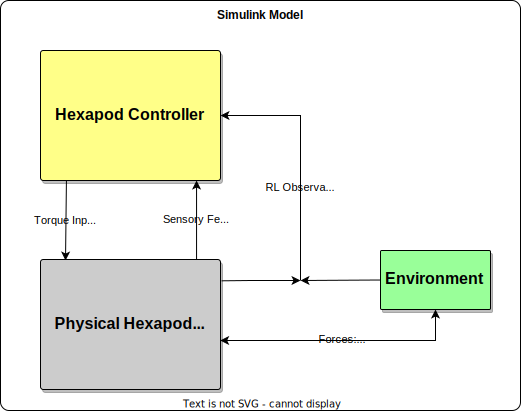
\includegraphics[scale=0.035]{HexapodModel_Overview}}
	\caption{Simulink Model Overview}
	\label{figure: Simulink Model Overview}
\end{figure}

Taking a top-down perspective on the Simulink model as depicted in \ref{figure: Simulink Model Overview}, it is distinctly divided into 3 separate components, the hexapod, the controller and the environment.
Being responsible for conducting the hexapods movement, the controller is, on a abstract level, responsible for deciding on the the speed, gait and direction of the robots movements.
On the lowest level this is accomplished by instructing the hexapod which torque has to be applied to each of its joints. 
The hexapod and the environment represent the components which physically interact with each other during the simulation.
Responding upon the commands received by the controller, the hexapod applies the torque values at each simulation step and returns sensory feedback to the controller.
This feedback is then used to adjust the commands which the controller will send during the next time step.
The hexapod takes all of these actions inside of the environment, all while interacting with it.
Additionally, if a RL agent is supposed to be trained, both the hexapod and the environment provide specific observations to the controller, which are used as inputs to the agent or to compute the reward function. 


\subsection{Model of the Hexapod}
The hexapod model we develop in this thesis is based on the \textit{PhantomX MK4} hexapod distributed by \textit{Trossen Robotics}.
The company provides a digital model of this robot in the form of an .urdf file which can be obtained from their Github page \parencite{interboticsGithub}.
URDF (\textbf{U}nified \textbf{R}obotics \textbf{D}escription \textbf{F}ormat) is a common file format for describing the physical and kinematic properties of a robot or robotic component.
It provides a standardized and structured way to define the connections between joints and links, the visual properties and collision geometry of each link as well as parameters such as mass and inertia \parencite{matlabURDFDocumentation}.
The geometry is provided in a separate folder in the form of CAD-files which are then referenced by the urdf.

The \textit{PhantomX MK4} follows the common architecture mentioned in \ref{sec: Hexapods}, meaning each leg has 3 joints and segments, totalling 18 DoFs.
Concerning the joint orientations, the \textalpha-joints movement plane lies is parallel to the ground while the \textbeta- and \textgamma-joint are restricted to a plane perpendicular to the ground, also in accordance to mentioned architecture.
The robot is axisymmetric towards its central axis(pointing in the movement direction) and the front and hind leg pairs are equally spaced from the middle leg pair.
The middle legs are attached to the thorax slightly further away from the central axis than the front and back legs.
A 3D model of the hexapod can be seen in Fig. \ref{figure: PhantomX 3D model}.

To import the model into the Simulink environment, we us a MATLAB-provided function to convert it from a urdf-file into a Simulink block diagram.
This process works automatically and results in a physically accurate Simulink representation without having to manually re-model the robot.
The representation consists of blocks from the Simscape library, more specifically joints, rigid transforms and coordinate frames to describe the robots kinematic chains, and rigid bodies to represent the individual links geometry and physical parameters.

\begin{figure}[h]
	\begin{subfigure}{.5\textwidth} % this sets the figure to be max half the width of the page
		\centering
		% include first image
		\includegraphics[width=.9\linewidth]{PhantomX_MK4_SideView}  % this sets the image to fill 90% of the available space -> 45% of the line width in total. 
		\caption{}
		\label{figure: PhantomX Side View}
	\end{subfigure}
	\begin{subfigure}{.5\textwidth}
		\centering
		% include second image
		\includegraphics[width=.9\linewidth]{PhantomX_MK4_FrontView}  
		\caption{}
		\label{figure: PhantomX Front View}
	\end{subfigure}
	
	\label{fig:fig}
	\begin{subfigure}{\textwidth}
		\centering
		% include third image
		\includegraphics[width=.45\linewidth]{PhantomX_MK4_TopView}   % this width should be half of the width of the other two images
		\caption{}
		\label{figure: PhantomX Top View}
	\end{subfigure}
	\caption[]{3D model of Trossen Robotics PhantomX MK4}
	\label{figure: PhantomX 3D model}
\end{figure}
\todo{get each image into list of figures, but exclude complete figure}

To be able to use the imported hexapod as a development platform we have to modify and expand the raw Simulink model as it does not provide any means to control it or receive feedback.
We reorganise and encapsulate logical groups, specifically the thorax and the individual legs, into library subsystems.
This enables us to propagate changes faster, as we only have to edit the library component instead of each existing instance.
As a side effect, this given the Simulink model a much more cleaned up and easier to understand appearance.
To be able to control each joint and receive sensory feedback from it, we enable the so called \textit{direct torque input} as well as the \textit{position} and \textit{acceleration} sensor readings on each joint block.
Trying to prevent increasing the models complexity to quickly, we do not model the physical servo motor attached to each joint and instead use the instantaneous torque application.
the joint block also allows for physical parameters to be modified, such as internal friction, dampening or spring stiffness.
We combine the 3 torque values and position/ acceleration readings of each leg into an input and output bus signal.
A view inside of the leg subsystem is given in \ref{figure: Hexapod Leg}, the subsystem block itself with its torque input and sensory feedback output buses can be seen in \ref{figure: Hexapod Model Overview} as part of the complete hexapod model.

\begin{figure}[h]
	\centerline{\includesvg[scale=0.55]{Simulink/Simulink_PhysicalHexapodOverview}}
	\caption{Overview of the Simulink Hexapod Model}
	\label{figure: Hexapod Model Overview}
\end{figure}

\begin{figure}
	\centerline{\includesvg[scale=0.5]{Simulink/Simulink_HexapodLegOverview}}
	\caption{Simulink model of the Hexapod Leg subsystem}
	\label{figure: Hexapod Leg}
\end{figure}

To enable the robot to physically interact with its surroundings, we enable the collision geometry on each of the models rigid bodies.
In Simscape, collision modelling involves establishing connections between a rigid body, and any other rigid body it should be able to interact with in a collision scenario, via Simscapes's \textit{Spatial friction force} block.
The block allows to modify the coefficients of static and dynamic friction, elasticity and dampening.\todo{does dampening exist in block ?}
An example of how this block can be utilized is shown in \ref{figure: Simscape Bouncing Ball Example}.
As collision detection is computationally relative expensive, we refrain from modelling robot self collisions and focus only on the interaction between robot and environment.
This means that the hexapods links can only collide with the ground plane but not with each other.
We realise this can potentially create discrepancies between simulation and real world, but as we initially only model predefined leg trajectories, which can be proven to not intersect, we are willing to give up a bit of realism in favour of faster simulations.

From a top level perspective, the modified robot model is represented by a single \textit{Hexapod} subsystem block, which receives the torques to be applied as input and outputs sensory information about each joint.
All of the internal joint parameters and friction coefficients used to model collisions are given in the tables \ref{table: Joint parameters} and \ref{X}.
The joint parameters were already mostly given by the urdf specification, while we adapted other parameters from \parencite{AUTHOR} and \parencite{AUTHOR2}.
\todo{Find source again}
To summarize, we converted the provided hexapod model into a Simulink model, compartmentalized it and added sensing and actuation capabilities to the robots legs.
In addition we made most of the models internal parameters accessible and modifiable within the MATLAB-script \textit{simulationsetup.m}.



\begin{comment}
The  thorax is represented by a rigid body and a main coordinate frame.
Each of the robots legs consists of 3 rigid bodies(coxa, femur and tibia) which are connected to each other by 2 joints.
A third joint then attaches the coxa and the leg as a whole to the main body.
Like the leg of an insect, the movement plane of the joint connecting coxa and thorax is parallel to the ground and orthogonal towards the other two joints.
Each of the joints used has 1 (rotational) DoF.
To position each rigid body and joint correctly, rigid transformations are used to translate and rotate each component.

As mentioned above, joints can receive as input a torque to be applied and can output sensory data, such as the joints position, velocity and acceleration. 
\end{comment}


\begin{table}
	\centering
	\begin{tabular}{| l | c |}
		\hline
		\textbf{parameter} & \textbf{value} \\
		\hline
		spring stiffness & 0 \\
		\hline
		damping coefficient & 0 \\
		\hline
		spring stiffness (joint boundary) & $10^4 \frac{Nm}{\text{deg}}$ \\
		\hline
		damping coefficient (joint boundary) &  $10 \frac{Nm \cdot s}{\text{deg}}$\\
		\hline
		transit region width (joint boundary) &  $10^{\circ}$\\
		\hline
	\end{tabular}
	\caption{Internal joint parameters}
	\label{table: Joint parameters}
\end{table}


%In this thesis we only utilize the sensor information about the current joint positions, but to allow for further expansions on the model, such as optimizing for minimal energy consumption, joint velocity and acceleration are provided as well.
%It should be noted, that integrating the joint position over time would implicitly yield the same result, but we decided for ease of use to include this data explicitly.


\subsection{Environment}
To validate the hexapod model and to provide a place for the robot to learn coordination strategies for its legs, we construct a simple test environment.
The environment at this point only consists of a horizontal plane, but can expanded to include more complex terrain with little effort.
Some examples which we experimented with, but did not utilise for testing or training so far, include inclined planes and also small obstacles on the ground.
As Simscape itself only provides basic geometric objects but allows for the use of .stl files to define the shape of objects, complex terrain such as irregular, uneven surfaces can be imported with relative ease.

In addition to being the testing ground of the hexapod model, the environment also acts as part of the reinforcement learning process.
Similar to \ref{figure: RL Illustration}, the environment provides observations to the RL agent and calculates a reward signal, based on the agents performance \todo{As of now not represented in the model, reward is part of controller}.
It does not however directly receive actions from the agent, as the hexapod, to which the actions are applied to by the RL agent, is its own subsystem.
If we would define the environment in a manner analogous to \ref{figure: RL Illustration,}, we would have to include both the environment subsystem and the hexapod subsystem as part of the "RL" environment.
For obvious reasons such as modularity and clarity of model we choose not to adapt this.

\subsection{Controller}
The controller is responsible for the hexapods locomotion.
It controls the movement of the robots legs according to an internally defined gait pattern.
As inputs, the controller receives the sensor data from the hexapod model.
According the internally defined gait pattern and the received data input, the controller outputs the torques to be applied to each joint of the hexapod.
The controller subsystem can be described as a feedback control system, as it receives feedback from a process it has to control and takes this feedback into account when generating new commands to steer the process.

\begin{figure}
	\centerline{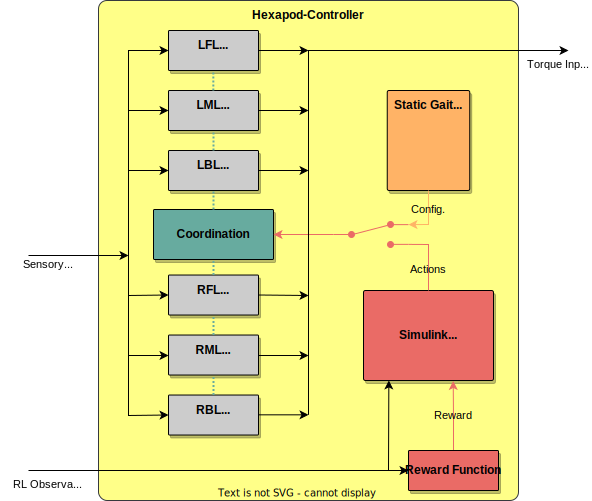
\includegraphics[scale=0.03]{HexapodController}}
	\caption{Controller Overview}
	\label{figure: Controller Overview}
\end{figure}

A depiction of the controller subsystem can be seen in Fig. \ref{figure: Controller Overview}.
As the legs move independently from one another, it consists of 6 separate control units, each responsible for controlling one of the six legs.
These units receive sensory information from the leg joints as input and compute the torques to be applied to the joints as output.
A legs control unit receives the desired frequency of the swing-stance cycle ($f_{c}$), the duty-cycle percentage ($P_{swing}$) and the swing-initiation signal ($s_i$) as coordination inputs.
The frequency $f_{c}$ defines how often the swing-stance cycle should be repeated per second, $f_{c} = 0.5 \text{ Hz}$ for example corresponding to one cycle every 2 seconds.
$P_{swing}$ describes the proportion of the swing (duty) phase in relation to a whole cycle and can be expressed by: 
\[
P_{swing} = \frac{T_{SW}}{T_{ST} + T_{SW}}, 
\] 
where $T_{sw}$ is the swing time and $T_{st}$ the stance time \parencite{qiu2023adaptive}.
A 50\% duty cycle would correspond to swing and stance being of equal length, both taking up exactly half a cycle time.
The swing initiation signal $s_i \in \{0,1\}$ notifies the control unit whether to initiate the swing phase ($s_i = 1$), independent of the legs position in the cycle, or whether to continue with the current cycle's execution ($s_i = 0$).
The controller also receives an additional input, a vector pointing in the direction the robot is supposed to move.
All these inputs can either be received from a static gait definition, in which the parameters for each leg are statically configured, or can be provided by a reinforcement learning agent.

The Simulink RL Agent, which is a separate component in the controller subsystem, receives observations from the environment and hexapod model as well as a reward signal and outputs an action vector which consists of similar commands as the static gait definitions commands.
The RL agent is a standard from the \textit{Reinforcement Learning} library and represents an agent in the same sense as described in \ref{sec: Reinforcement Learning}.
The RL agent and reward function will be detailed more precisely in section \ref{sec: RL setup}.

\begin{figure}
	\centerline{\includesvg[scale=0.6]{Simulink/Simulink_LegControllerOverview}}
	\caption{Control unit for a single leg}
	\label{figure: Leg control unit}
\end{figure}

Continuing  with the explanation of the controller subsystem, we now focus on a single leg control unit.
Such a unit, as can be seen in \ref{figure: Leg control unit}, consists of a leg trajectory generator and 3 PID feedback control loops, one for each of the leg joints.
The leg trajectory generators task is to generate joint angles which allow the leg end-effector to follow a smooth trajectory, all in accordance to the input frequency, duty cycle, swing initiation and pattern rotation.
At each time step it outputs the desired angle for the \textalpha-, \textbeta- and \textgamma-joints, which the PID controllers then work on achieving by regulating the applied torques.
The PID controller parameters $K_p$, $K_i$ and $K_d$ (and $N$) are tuned via trial-and-error method and are given in \ref{table: PID parameters}.

\begin{figure}
	\centerline{\includesvg[scale=0.75]{Simulink/Simulink_LegTrajectoryGenerationOverview}}
	\caption{Leg trajectory generator}
	\label{figure: Leg trajectory generator}
\end{figure}

The leg trajectory generator, as seen in \ref{figure: Leg trajectory generator}, consists of a signal generator, a pattern rotation subsystem and an analytical inverse kinematics solver.
The signal generator is responsible for creating a continuous leg trajectory in the form of 2-dimensional trajectory coordinates.
The pattern rotation subsystems applies, if required, a simple mathematical rotation to  the planar trajectory(x,z-plane) around the z-axis to allow for omni-directional movement of the robot.
Finalizing the trajectory generation, the inverse kinematics solver receives the trajectory coordinates and translates them into the \textalpha, \textbeta and \textgamma joint angles.


\subsubsection{Analytical Inverse Kinematics Solver} \label{subsubsec: IK Solver}
Even though Simulinks \textit{Robotics System Toolbox} includes an iterative IK-solver, we decided to implement our own analytical solver.
Early in the development process, we realized that the iterative solver provided would not be sufficient for our intended purpose.
Due to the nature of iterative solution methods, the calculation time required to find a valid configuration is significantly higher than that of a purpose-build analytical solver and thus greatly increased simulation times.
As we need to simulate several thousand episodes during reinforcement learning, we aim to minimize the 
amount of time required to compute a time step in the simulation.

The solver sequentially calculates the 3 joint angles of a leg, starting at \textalpha, then \textbeta and \textgamma.
The solver is derived from the legs geometric properties as seen in \ref{figure: IK angle derivations}

\begin{figure}[h]
	\begin{subfigure}{.5\textwidth} % this sets the figure to be max half the width of the page
		\centering
		% include first image
		\includegraphics[width=\linewidth]{IK_Solver_alphaAngle}  % this sets the image to fill 90% of the available space -> 45% of the line width in total. 
		\caption{}
		\label{figure: IK Solver Alpha Angle}
	\end{subfigure}
	\begin{subfigure}{.5\textwidth}
		\centering
		% include second image
		\includegraphics[width=\linewidth]{IK_Solver_betaGammaAngle}  
		\caption{}
		\label{figure: IK Solver Beta/Gamma Angle}
	\end{subfigure}
	\caption[Angle derivation drawings]{(a) Top-down view of a hexapod leg, used to determine \textalpha. (b) Side-view, used in the in the determination of \textbeta \ and \textgamma.}
	\label{figure: IK angle derivations}
\end{figure}


 Given the length of each leg segment, the 3 angles are calculated as following:

\[
	\alpha = \arctan(\frac{x}{y}) ,\quad \quad \quad \beta = 90^{\circ} - (\beta_1 + \beta_2) ,\quad \quad \quad \gamma = 90^{\circ} - \gamma_1.
\]
\\
Where $\beta_1$, $\beta_2$, $\gamma_1$ and \text{BF} are given by:
\[	
	\beta_1 = \arccos(\frac{{l_\text{femur}}^2 + \text{BF}^2 - {l_\text{tibia}}^2}  {2\cdot l_\text{femur} \cdot \text{BF}}) ,\quad \quad \quad \beta_2 = \arctan(\frac{ l_\text{total} - l_\text{coxa}} {z}),
\]

\[
	\gamma_1 = \arccos(\frac{{l_\text{tibia}}^2 + {l_\text{femur}}^2 - {\text{BF}}^2}  {2 \cdot {l_\text{tibia}} \cdot {l_\text{femur}}}) ,\quad \quad \quad \text{BF} = \sqrt{(l_\text{total} - l_\text{coxa})^2 + z^2}.
\]








\begin{figure}[h]
	\centerline{\includesvg[scale=0.85]{Simulink/Simulink_SignalGeneratorOverview}}
	\caption{Signal Generator}
	\label{figure: Signal Generator}
\end{figure}

A Signal Generator, as seen in \ref{figure: Signal Generator}, consists two parts, a swing phase subsystem and a stance phase subsystem.
The stance subsystems provide the x- and z-coordinate signal during stance, the swing subsystem during swing.
The coordination between these two units is influenced by the cycle frequency, duty factor and swing initiation signal.
If the swing initiation is pulled high, the swing phase subsystem is reset(so it starts from the beginning) and the outputs(x,z) are switched to the swing system.
When the swing phase is finished, meaning the x-coordinate coincides with the AEP, the swing phase subsystem gives up control the the stance phase subsystem via the \textit{Swing finished} signal.
This induces a reset on the stance phase subsystem and switches the outputs over to this system.

\begin{figure}
	\centering
	\begin{subfigure}[b]{0.55\textwidth}
		\includesvg[width=1\linewidth]{Simulink/Simulink_SwingPhaseGenOverview}
		\caption{}
		\label{fig:Ng1} 
	\end{subfigure}
	
	\begin{subfigure}[b]{0.55\textwidth}
		\includesvg[width=1\linewidth]{Simulink/Simulink_SwingPhaseGenOverview}
		\caption{}
		\label{fig:Ng2}
	\end{subfigure}
	
	\caption[Swing and Stance Phase]{(a) Swing phase subsystem. The swing ellipse is generated by two sine waves with different amplitude and phase. (b) Stance phase subsystem. As opposed to (a), the x-coordinate is now generated by a linear function and the z-coordinate is 0 throughout the whole phase.
		values of $M,I$.}
\end{figure}




\begin{table}[h]
	\centering
	\begin{tabular}{| c | c |}
		\hline
		parameter & value\\
		\hline
		$K_p$ & ... \\
		\hline
		$K_i$ & ... \\
		\hline
		$K_d$ & ... \\
		\hline
		$N$ & ... \\
		\hline
	\end{tabular}
	\caption{Gain parameters used for pid-tuning}
	\label{table: PID parameters}
\end{table}

\begin{table}
	\centering
	\begin{tabular}{| c | c | c | c |} 
		\hline
		 & \textbf{\textalpha} & \textbf{\textbeta} & \textbf{\textgamma} \\ [0.5ex] 
		\hline
		left front, right back & 45 & 14.03624347 & 60.58440117  \\ 
		\hline
		left/right middle & 0 & 14.03624347 & 60.58440117 \\
		\hline
		right front, left back & -45 & 14.03624347 & 60.58440117 \\
		\hline
	\end{tabular}
	\caption{Initial joint positions according to urdf-file}
	\label{table:Initial joint positions}
\end{table}

For spatial contact force parameters, see \parencite{trotta2022walking}.

When running the simulation at large step sizes, we observed simulation instabilities similar to the ones mentioned in \parencite{thilderkvist2015motion}, although not of the same significance.
We attribute the unsatisfactory results they experienced from the spatial friction forces to be most-likely linked to an earlier MATLAB version used for their work.
A step size of 0.00025s(0.25ms) resulted in satisfactory behaviour in almost all of our simulations.
Only when training a RL agent, we reduced the step size initially even further to anticipate uncoordinated, trembling behaviour due to an untrained agent.


\section{Learning Leg Coordination} \label{sec: RL setup}
The leg coordination problem can be considered a Markov decision process(MDP).
The MDP is a 5-tuple $\mathcal{\{S,A,P,R,\gamma\}}$, where $\mathcal{S}$ is a finite set of states, $\mathcal{A}$ is a finite set of actions, $\mathcal{P}$ is a state-transition probability matrix ($\mathcal{P}_{ss'}^a=\mathbb{P}[S_{t+1}=s' | S_t=s, A_t=a]$), $\mathcal{R}_s^a$ is a reward function ($\mathcal{R}_s^a = \mathbb{E}[R_{t+1} | S_t=s, A_t=a]$) and $\gamma \in [0,1]$ is a discount factor.


When we first started working on te RL process, te result were not very promising. The agent did stabilize, meaning it did not jump around randomly, but it was not able to find an efficient gain.
The agent never learned to reliably move a leg forward if it was start to drag behind due to reaching the PEP.

The reward stayed relatively flat over a period of over 2000 episodes of training.
The strong deviation from the mean, even after several hundred episodes can be attributed to an averaging window of just 5 episodes(or steps ?). 
In later training experiments, this averaging window was increased.
The small averaging window might have contributed to the poor performance of the agent(unlikely, olny important for average graph ?).

MATLABs Reinforcement Learning Toolbox offers several different RL architectures to choose from, namely DDPG, TR3, PPO, SAC and TRPO.
We choose to use the DDPG as well as PPO algorithms, as these have already proved themselves to work well in tasks concerning robotic locomotion\parencite{FIND AUTHOR}.
\todo{Find authors who used DDPG and PPO for robotics(PPO bei Schilling(?), DDPG bei ? )}




DDPG does not jitter at start of learning, PPO does.

To speed up the learning process, we decided to utilize \textit{MATLABs Parallel Computing} toolbox.
The toolbox allowed us to create a parallel pool of several workers, each of whom runs a separate episode of the RL process.
The parallel learning process is carried out asynchronously, meaning workers who finished their task early do not have to wait on the others to finish as well before proceeding.
In contrast to synchronous parallelization, where the workers send their results to the parallel pool client all at the same time and receive updates to their parameters all at once, workers under asynchronous parallelization can send their results as soon as they finish their task and instantly receive parameter updates.
By parallelization, we significantly improve the number of simulated episodes.



Start learning process of PPO(Proximal Policy Optimization) agent at a small step size(0.00025s = 0.25ms) to prevent simulation errors due to initial random jerking of robot legs.
After the agent has stabilized, the step size can be increased to speed up the further learning process.]


Observation space only consists of a part of all states, thus the MDP can not be fully described and is therefore called a Partially Observable Markov Decision Process(POMDP).
The robot could be equipped with additional sensors to perceive a larger part of the state-space, but we find that the observations given by us are sufficient for successful learning of the defined task.


\cite{lillicrap2015continuous}
\todo{Describe dimension of action and observation space}





\textbf{Optionals:}

\begin{itemize}
	\item Signal the agent that a leg is dragging by adding a discrete observation per leg which is pulled high when the leg reached its PEP.
	
	\item Add more inputs to the RL agent
	
	\item Agent Parallelization for faster learning $\rightarrow$ Done and working
	
	\item RL Designer: Automatically save agents which reached a high enough reward to evaluate them later $\rightarrow$ Done.
	
	\item As we have multiple robotic 'actuators' in this project, a continuous action space is favorable.
	
\end{itemize}





\end{titlepage}

\begin{titlepage}
	%!TEX root = ../thesis.tex
\chapter{Results}
\label{ch:results}

In this chapter we present the results we compiled during the course of our work.
This includes an evaluation of the developed hexapod model and its locomotion controller, as well as review of the RL training results obtained and lessons learned from observing the training process.

\section{Evaluation: Hexapod model}
During the development process of the hexapod model and locomotion controller, we observed that the conceived modular architecture enabled us to quickly modify and/or add components.
An example of this flexibility is provided by the retrospective addition of sensor readings for the rotational acceleration of the \textalpha-joints.
As the hexapod leg is defined as a library component, it was only necessary to enable the respective sensor reading one the joint block and add the new signal to the already existing sensory information bus. 
There was no need to modify the hexapods legs individually, as Simulink automatically updates all library-linked blocks.
In general, the library of custom subsystems has proven to be a most useful tool, reducing development time and promoting modularity.
The encapsulation of the hexapod model as a whole into a single, top-level subsystem block, that only reveals necessary in- and outputs, provides the developer with a simple to understand interface.
It also gives us the ability to duplicate the complete hexapod system without any effort, which could prove useful in future research as it enables the system to easily be utilized in multi-agent simulations.

Concerning the actual simulation of the model, it can be said that in most cases in which the robot uses a statically defined gait pattern for locomotion, a simulation step size of 0.5 ms yields stable results and runs at close to real time.
Given an untrained, exploring RL agent as the models operator, a step size of 0.25 ms is preferable, as sudden twitching and jerking motions might occur, which can lead to simulation instabilities and exceptions.
Similar to the results of \cite{thilderkvist2015motion}, we begin to observe these problems at larger step sizes ($> 0.5 ms$), although not of the same significance and frequency as described by them. 
The most common reason for exceptions we observed, were collision detection failures.
These occur, when two rigid bodies move into each other faster than the simulation's solver can observe, due to its limited temporal resolution.
During the several ten-thousand simulation episodes performed at a step-size of 0.25 ms during RL training, we did not once observe an exception.
Overall, the behaviour of our robot model seems, to the best of our knowledge, but without the co-examination of a real world counterpart, physically accurate.


We attribute the unsatisfactory results \cite{thilderkvist2015motion} experienced from the spatial friction forces to be most likely linked to deciding on a step size too large for stable simulations.
As they also work with an earlier MATLAB version, using Simscape's predecessor \textit{SimMechanics}, the problems might also have arisen from a possibly more primitive physics model.

To summarize, we were able to create a well-functioning, virtual model of a hexapod robo in Simulink.
Simulations of the model are robust, physically accurate and performant.
Utilizing a modular architecture, the model can easily be adapted to changing requirements.
 

\section{Evaluation: Locomotion Controller}
The locomotion controller we presented in \ref{subsec: Locomotion controller} is the result of several design iterations.
We extensively tested each of the designs to uncover their weakpoints, upon which the next iteration was improved on.

To begin with, the initial design (\textit{MK1}) enabled the robot to walk in a straight line tripod gait.
We observed that the hexapod model, controlled by MK1, would jerk up and down significantly during a movement cycle, as can be seen in [\hyperref[vid: MK1]{MK1}] and \ref{figure: Thorax Height graph, bad tuning}.
During a legs swing phase, the robot's thorax would slowly sink towards the side of the lifted leg and be rapidly pushed upwards again at the end of the swing.
As we defined the leg trajectory relative the thorax and did not consider sensing ground contact or body tilt, the leg on the sinking side would hit the ground earlier than expected by the controller, as the anticipated AEP "sunk" into the ground plane.
We were able to later on attribute this behaviour to the slow reactions of the PID controllers.
These were, given our initial tuning parameters ($K_p = 3, K_i = 0.2, K_d = 1, N = 100$), unable to follow their assigned trajectories. 
In addition, the MK1 controller version requires a lot of calculation time per simulation step, resulting in slow simulations.
The observed cause of this being the computationally intensive, iterative IK block provided by Simulink, as we have already elaborated on in \ref{subsubsec: IK Solver}.

With the subsequent design iteration \textit{MK2}, we focused on introducing tetrapod and wave gait as well as increasing simulation speed.
Implementing the gait patterns proved to be straightforward, as, resulting from the modular architecture, solely the leg coordination of the static gait definition had to be modified.
The resulting simulations of the robot walking in tetrapod and wave gait can be observed in [\hyperref[vid: MK1]{MK2}].

The decision to implement our own, custom analytical IK solver yielded a significant performance boost.
Comparing the MK1 and MK2 controllers, we are able to achieve an up to 5x speed up in simulation time.
Running a 30 second simulation of a hexapod walking in tripod gait, controlled by MK1, required a full 143 seconds of real compute time, while the same simulation takes about 38 seconds to run when the hexapod is controlled by MK2.

With the final non-RL controller design, termed \textit{MK3}, we improved the stability of the hexapods locomotion as well as introduced the capability for omnidirectional movement.
By simply re-tuning the PID controller parameters to the values displayed in \ref{table: PID parameters}, we were able to reduce the jerking behaviour of the robot far enough to almost not being visually noticeable.
A comparison of the thorax's height differences during movement, when under control of the MK2 and MK3 controllers, can be seen in Fig. \ref{figure: Thorax height graphs}.


\begin{figure}[h]
	\begin{subfigure}{\textwidth} % this sets the figure to be max half the width of the page
		\centering
		% include first image
		\includegraphics[width=.9\linewidth]{ThoraxHeight_firstPID.PNG}  % this sets the image to fill 90% of the available space -> 45% of the line width in total. 
		\caption{}
		\label{figure: Thorax Height graph, bad tuning}
	\end{subfigure}
	
	\begin{subfigure}{\textwidth}
		\centering
		% include third image
		\includegraphics[width=.9\linewidth]{ThoraxHeight_retunedPID.PNG}   % this width should be half of the width of the other two images
		\caption{}
		\label{figure: Thorax height graph, re-tuning}
	\end{subfigure}
	\caption[Thorax height graphs]{(a) Thorax height graphs of hexapod robot controlled by (a) MK2 and (b) MK3 controller.}
	\label{figure: Thorax height graphs}
\end{figure}

Our final, MK3 locomotion controller is able to control the hexapod model in tripod, tetrapod as well as wave gait.
The swing-stance cycle frequency ($f_c$) and the duty cycle percentage ($P_\text{swing}$) can be changed, even dynamically during simulation.
We demonstrate this dynamic frequency alteration with a hexapod model walking in wave gait with varying cycle frequency.
The controller initiates movement with at $f_c = 0.1\ \text{Hz}$, slowly increasing over 20 seconds linearly to $f_c = 0.5\ \text{Hz}$. 
It is further also possible to redefine the step height and AEP/ PEP positions, opening up possibilities for more dynamic control algorithms.
As already mentioned, the final controller is capable of instructing omnidirectional movement, as we demonstrate in a study of the robot walking in a circle.
Additional studies of the hexapod robot performing all predefined gait patterns at different cycle frequencies were performed as well.
We captured all of the simulations mentioned above as videos which can be found at [\hyperref[vid: MK1]{MK3}].

Concerning the hexapods ability to navigate obstacles or uneven terrain, it has to be noted that the controller does not possess any means of observing environmental details.
It is not able to recognize obstacles in it's path and therefore struggles to overcome even small objects.
We explored the robots performance at traversing a 10 cm wide an 4 cm high beam, perpendicular to the robots movement direction.
Summarizing the findings of simulations in all available gaits, the hexapod walking in tripod gait was able to eventually overcome the obstacle, while it struggled to do so in both tetrapod and wave gait, given the allotted timespan of 60 s.
We attribute the tripod gait's success to the fact that it presents the lowest number of legs in stance at any point in time, as we observed that legs in stance often get caught on the obstacle.
Due to the nature of our controller, legs in their stance phase are rather reluctant to deviation from their trajectories.
Thus, when caught in from of the obstacle, they prevent the robot from moving forward.
Videos of the obstacle traversal simulations can be observed in [\hyperref[vid: MK1]{MK3}].


\section{Evaluation: RL training}

Implementing a RL agent yielding satisfying results proved to be more difficult than anticipated.
As there exists a large set of parameter to be considered during setup, finding a well-performing set has shown to be a time-consuming task.
This was reinforced by the fact that, to observe the performance of a set of parameters, we found an agent required at least 1-2 k episodes of training, equating to several hours of runtime given the hardware used.
Additionally, as we ran experiments with two different RL algorithms, we were required to tune two separate sets of parameters.
In total, we trained over 30 different agent configurations.
As we are not able to present all the results obtained, a table providing information on all documented configurations is included in the appendix (\emph{\nolinkurl{RL_agent_configs.xlsx}}).\\
In the following sections, we will present the findings obtained from the performed RL training experiments, focusing on a selected subset of training runs.

\subsection{Reward Exploitation}
A general problem, which is often observed in RL, is an agent exploiting a poorly-defined reward function \parencite{silver2015}.
This commonly leads to agents exhibiting undesirable behaviour, even though according to the reward function they are performing well.
We experienced this exploitation behaviour during development as well.
As our reward function initially did neither take into account the robots energy consumption ($W$) nor height differences of the thorax during movement ($ \Delta_h$), early RL agents exploited this simpler reward function by learning to jump.
More specifically, we observed the robot to exhibit a behaviour consisting of small, abrupt hops, using it's hind legs to propel itself forward.
We provide a recording of the observed behaviour in [\hyperref[vid: MK4]{MK4}], the training graph of the agent can be seen in \ref{}.
In the graph, the occurrence of the exploit is clearly visible as a spike in the average reward that quickly breaks down again.

In the further development process, we refined the reward function weights and included $W$ and $\Delta_h$ to encourage the RL agents to be more resourceful. 
Our final reward function weights, with which we obtained the most promising results, are displayed in table \ref{table: Reward weights}.


\subsection{Learning Behaviour}
The phenomenon of sharp spikes in the average reward as mentioned above, persisted throughout our training runs, repeating on several different agent configurations.
A training graph depicting this behaviour can be seen in Fig. \ref{}.
We suspect these reward plunges to be related to the agent exploring too rapidly/ changing it's policy to fast, resulting in a loss of the already achieved progress \parencite{silver2015}.
However, were cannot provide a definite prove of this cause, as we are not able to reliably prevent the behaviour from occurring.
On the other hand, in stark contrast to the phenomenon just explained, we also observed "flatlining" of the average reward.
An agent would often learn well initially, but after a certain number of episodes converge to an average reward well below that of individual episodes.
Interestingly, this behaviour could very well be attributed to the agent's policy updates not being large enough, such that it is unable to leave a locally optimal policy only based on a few episodes of high reward \parencite{silver2015}.
Despite our efforts to find a middle ground between these two extremes by changing the agent's learning rate an introducing varying amounts of randomness into it's decision process, we were not able to find a well-working configuration.


\subsection{Best Result}
Given the reward function weights in table \ref{table: Reward weights}, a sample rate of 0.05 s and an episode length of 256 steps, the best result we were able to achieve with an RL agent was a maximum episodic reward of 310 units.
In this training run, performed with a DDPG agent with parameters listed in \ref{table: DDPG parameters}, the average reward did neither spike nor converge to a suboptimal policy, as can be seen in \ref{}.
Even though, the average reward does not seen to reliably increase.
Observing the agent's performance in simulation, it's behaviour does not seem to constitute a stable gait pattern.
The hexapod uses various legs to slowly push itself forward, seemingly uncoordinated.
The agent appears to be unable to notice a leg finishing it's stance phase, as often several legs drag behind, due to them reaching the PEP and not being lifted back up again.
A demonstration of the best performing policy obtained from this training run, can be seen in [\hyperref[vid: MK4]{MK4}].
Comparing this result with a hexapod walking in a statically defined tripod gait, which obtains a reward of $\sim785$ units given the same sample rate, episode length and steps, the RL policy performs about 40\% as well as the static gait.


{\def\arraystretch{1.4}\tabcolsep=5pt
	
	\begin{table}[h!]
		\parbox{.4\linewidth}{
			\centering
			\begin{tabular}{| c | c |} 
				\hline
				\textbf{Training params.s} & \textbf{Value} \\ [0.5ex] 
				\hline
				\hline
				Sample time & 0.05 s \\ 
				
				Episode steps & 512 \\
				
				\hline
				\textbf{Agent params.} &  \\ [0.5ex] 
				\hline
				
				Learn Rate & $\num{3e-4}$ \\
				
				Episode steps & 512 \\
				
				Exp. Buf. length & $\num{1e6}$ \\
				
				Discount factor &  0.99 \\
				
				Mini-Batch size & 32 \\
				
				NN-width & 128 \\
				
				\hline
				\textbf{Noise params.} &  \\ [0.5ex] 
				\hline
				
				\textsigma\footnote{\textsigma: Standard Deviation} & 0.05 \\
				
				\textsigma-decay\footnote{\textsigma-decay: Decay rate of \textsigma. Each sample time step k, \textsigma decays according to following formula: $\sigma_{k+1} = \sigma_k \cdot (1 - \textbf{\textsigma-decay})$} & 1e-6 \\
				
				\hline
			\end{tabular}	
			\caption[DDPG agent parameters]{}
			\label{table:DDPG parameters}
		}
	\end{table}
}

{\def\arraystretch{1.4}\tabcolsep=5pt
	\begin{table}[h!]
		\centering
		\begin{tabular}{| c | c |}
			\hline
			\textbf{Weight} & \textbf{Value}\\
			\hline
			\hline
			$c_{s_x}$   		&  1	\\
			$c_{v_x}$   	    &  50	\\
			$c_{v_y}$  		    &  1	\\
			$\Delta_h$  		&  1	\\
			$c_W$ 				&  0.025\\
			\hline
		\end{tabular}
		\caption[Reward weights]{}
		\label{table: Reward weights}
	\end{table}
}



\subsection{Further Remarks}
As we changed the reward function several times in attempts to improve it's ability to accurately describe the performance of an agent, the individual training results can only be compared to a limited extend.
Concerning the two policy optimization algorithms used, DDPG and PPO, there were no significant differences in their performance to be observed.
We therefore abstain from comparing the algorithms separately.

%We used the \textbf{D}eep \textbf{D}eterministic \textbf{P}olicy \textbf{G}radient (DDPG) algorithm, an actor-critic, model-free, online, off-policy RL method.
%The actor network consists of a 12-wide observation input layer followed by 3 100 neuron wide fully-connected layer, in between each of them a ReLU-layer to introduce non-linearity.
%Concluding the actor network is an output layer consisting of 6 neurons, one for each action channel.
%The architecture of critic network is more complicated, as it has to take in more informations.
%At the start this network consists of two separate branches, one taking as inputs X and one Y.
%On both branches the input layers are followed by a fully-connected and a ReLU layer.
%At this point the two branches are connected by a simple addition layer.
%After the add-layer, another 2 combinations of fully-connected and ReLU layer follow, concluding with a single output neuron, representing the critics reward estimation.
%All of the actor and critic layers are, if not mentioned otherwise, 100 neurons wide.
%The architectures of the actor and critic networks have been adopted from example applications created by \cite{matlabDDPGExample, matlabPPOExample}.

%We used a learning rate of $3e^{-4}$ and $1e^{-3}$ for the actor and critic respectively and a discount factor of 0.99.
%The agents sample rate is set at 0.05, meaning the agent samples the environment and takes an action every 50 ms.
%A more detailed summary of the RL parameters is given in table \ref{table: DDPG parameters}.

{\def\arraystretch{1.4}\tabcolsep=5pt
\begin{table}
	\centering
	\begin{tabular}{| l | c |}
		\hline
		\textbf{Parameter} & \textbf{Value}\\
		\hline
		\hline
		Actor learn rate & $3e^{-4}$ \\
		Critic learn rate & $1e^{-3}$ \\
		Discount factor &  0.99 \\
		Mini-Batch-Size & 16 \\
		Experience buffer & $1e^6$\\
		\textsigma \ (UB) & 0.2 \\
		\textsigma-decay (UB) & $1e^{-6}$ \\
		
		\hline
	\end{tabular}
	\caption[DDPG parameters]{DDPG parameters. Uhlstein-Beck (UB) noise model is used to introduce noise into the agents exploration}
	\label{table: DDPG parameters}
\end{table}
}


\begin{figure}[h]
	\begin{subfigure}{\textwidth} % this sets the figure to be max half the width of the page
		\centering
		% include first image
		\includegraphics[width=\linewidth]{graphs/cropped/exploitGraph_cropped.PNG}  % this sets the image to fill 90% of the available space -> 45% of the line width in total. 
		\caption{}
		\label{figure: RL a}
	\end{subfigure}
	\begin{subfigure}{\textwidth}
		\centering
		% include second image
		\includegraphics[width=\linewidth]{graphs/cropped/firstSuccess_146reward_cropped.PNG}  
		\caption{}
		\label{figure: RL b}
	\end{subfigure} 
		\caption[Training graphs (1)]{Training graphs (1): Each graph depicts the learning curve of a RL agent. The dark blue graph represents the average reward over a running average of 250 episodes, while each data point on the light blue graph represents the reward obtained during a specific episode. (a) Jumping exploit learning curve. (b) Reward spiking.
		}
	\label{figure: DDPG learning graphs 1}
\end{figure}

\begin{figure}[h]
	\begin{subfigure}{\textwidth} % this sets the figure to be max half the width of the page
		\centering
		% include first image
		\includegraphics[width=\linewidth]{graphs/cropped/flatlining_cropped.PNG}  % this sets the image to fill 90% of the available space -> 45% of the line width in total. 
		\caption{}
		\label{figure: RL c}
	\end{subfigure}
	\begin{subfigure}{\textwidth}
		\centering
		% include second image
		\includegraphics[width=\linewidth]{graphs/cropped/lastAgent_graph_cropped.PNG}  
		\caption{}
		\label{figure: RL d}
	\end{subfigure} 
	\caption[DDPG training graphs (2)]{DDPG training graphs (2):  (a) Reward flatlining (b) lastAgent.}
	\label{figure: DDPG learning graphs 2}
\end{figure}


\subsection{Hardware}
The simulation studies and RL training runs were all performed on a desktop computer powered by an Intel i7-11700K CPU, 32 GB of RAM and a NVIDIA RTX 2060 GPU.
Concerning MATLAB, we used version 2023a for all of our work.


\end{titlepage}

\begin{titlepage}
	%!TEX root = ../thesis.tex
\chapter{Conclusion and Outlook}
\label{ch:conclusion}

In this concluding chapter, we summarize our key finding and contributions.
We discuss the value of the developed model as a foundation for future research and highlight the insights we gained into the task of applying RL to the problem of leg coordination.
Lastly, we provide an outlook toward potentially interesting future research topics, expanding on foundations established in our work.

\section{Conclusions}

MATLAB Simulink proved to be a versatile and reliable platform for the modelling and simulation of robotic systems.
The development of the hexapod model was greatly sped up by the underlying MATLAB framework and the utilisation of the provided toolboxes.
The ability to write MATLAB-scripts to automate several task, like the initialisation of the hexapod model or the setup of the RL agents and surrounding infrastructure, significantly increased our productivity.
We are confident that the developed model can serve as a platform for future research, as it utilizes a modular architecture, can easily be adapted to changing requirements and is based on the versatile MATLAB environment.
The model also proved surprisingly robust in the face of constant twitching caused by exploring RL agents.

Another benefit the use of MATLAB provided was the \textit{Parallel Computing Toolbox}. 
By being able to run 8-16 agents in parallel, one per processor core or multiple in separate threads, we were able to greatly increase the number of RL training episodes and thus faster reach conclusions on the examined agents.
As we were unsuccessful in creating an agent with an emergent gait, we can not speak to the effectiveness of continuing the training of already performant agents even loger.

As to the reasons for why the RL approach did not yield satisfying results, we have several potential explanations:
\begin{itemize}
	\item \textbf{Inadequate reward function: } As we already mentioned, defining a reward function which accurately judges an agent's performance is a difficult task, requiring expertise.
	Although we based our reward function on existing literature \parencite{trotta2022walking, schilling2021decentralized}, refined it's weight over several iterations and thoroughly tested it judgement on the static gait patterns, we cannot rule out a flaw in the function which leads to exploitation or loss of relevant information.
	
	\item \textbf{RL algorithm configuration: } Over the course of this work we experimented with many different RL parameters, many of which have already been successfully applied by other authors \parencite{matlabDDPGExample, matlabPPOExample, trotta2022walking}.
	Even so, there does not exist any literature on the same problem of leg coordination given a fixed leg trajectory and thus the possibility exists that we did not discover a performant set of parameters.
	As the learning ability of both policy optimization methods (DDPG, PPO) was observed to be about equal, we are however confident that the chosen algorithms are not the cause of the observed problems.
	
	\item \textbf{Continued Development: } As we continued to develop and improve both the locomotion controller and the RL setup while we were already training RL agents, there does not exist a fixed, final state of the underlying model, on which all training was based.
	The resulted of which is a limited comparability of the the trained agents.
	
\end{itemize}



We were unsuccessful in our task to train an agent which can perform a stable gait pattern.

We are confident that, given more time to carefully tune parameters and reward, the training time could be reduced significantly and performance improved.

We found the learning of the RL agents to progress quite slow. 
This could probably be improved on significantly by more carefully tuning the agents parameters and a more detailed reward function.



Our suggestions for future researchers attempting to apply RL to the leg coordination problems are the following:
\begin{enumerate}
	\item Do not change the underlying hexapod model during experimentation with different RL agents. 
	These changes make it difficult to compare the performance of RL parameter sets.
	The hexapod model should be meticulously tested prior to the application of RL.
	As our main goal was to provide the best-performing hexapod model, we decided to rather fix mistakes we discovered, sacrificing on comparability .
	
	\item Automate the process of running several agents with different parameter sets. 
	By automating this task, the speed of exploration in the parameter space could be greatly increased.
	
	\item Meticulously collect the data of each agent's performance to be able discover trends on which parameter values might work well.
	
\end{enumerate}

Given that the primary objective of this thesis was the creation of a functional and resilient hexapod model, serving as a foundational platform for future research, we consider our efforts a success.
In addition to the hexapod model itself, we successfully designed a basic locomotion controller and established a framework for applying RL to the hexapod system, offering potential starting point for future expansions.
In summary, the development of the hexapod model and locomotion controller can be deemed successful, while the approach to solving the RL leg coordination problem presents an ongoing challenge to which further research has to be applied.


\section{Outlook - Future Work}

In this last section, we draw our work to a close by suggesting possible future expansions to the model and more broadly point of future research interest.
As we also only implemented a rudimentary locomotion controller capable of navigation on flat terrain, expanding the controller's capabilities to more complex, uneven terrain would be a valuable research target.
Since the goal of successfully applying RL to the problem of leg coordination was not reached in completion, it might also be appealing, as a future work, to focus solely on this problem.
This could include a deeper investigation into reward function definitions and the task of tuning parameters of a RL algorithm.
Looking further ahead, a substantial research goal could involve applying RL to learn hexapod locomotion from scratch, granting the agent complete control over all 18 DoF.
In conclusion, while our current work lays a strong foundation on which further works can be based, it also reveals a range of unexpected difficulties to be explored in the future..


\begin{comment}

\begin{itemize}
	
	\item Controller improvements:
		\subitem Curve walking
		\subitem Adaptation to uneven terrain
		\subitem 
	
	\item Expand Reinforcement Learning from just leg coordination towards controlling the whole movement process
		\subitem Improve reward definition/ terminate episodes in which no progress seems to be made after some time(such as in \cite{lillicrap2015continuous})
		\subitem Learn walking from the ground up, meaning the agent controls each of the 18 joints (maybe take steps in between)
		\subitem
	
	\item Use other MATLAB Tools such as Hardware Co-Simulation to test controller on real robot
	
	\item 
	
\end{itemize}
\end{comment}
\end{titlepage}


\appendix % hier beginnt der Anhang
%\input{chapter/appendix_chapter.tex}
%\cleardoubleoddemptypage

\listoffigures
\cleardoubleoddemptypage

\listoftables
\cleardoubleoddemptypage

\printbibliography
%\cleardoubleoddemptypage
%!TEX root = ../thesis.tex
\chapter*{Declaration of Academic Integrity}
I hereby confirm that this thesis, entitled 

\begin{center}
	\textit{\printtitle}
\end{center}

is solely my own work and that I have used no sources or aids other than the ones stated. All passages in my thesis for which other sources, including electronic media, have been used, be it direct quotes or content references, have been acknowledged as such and the sources cited. I am aware that plagiarism is considered an act of deception which can result in sanction in accordance with the examination regulations.

\vspace{0.75cm}
\includegraphics[scale=0.35]{Signature_BastianKlein.png} \\
\parbox{17em}{\hrulefill} \\
\printname,
\printcity, \today
\vspace{0.75cm}
\par

I consent to having my thesis cross-checked with other texts to identify possible similarities and to having it stored in a database for this purpose.
\\
\\
I confirm that I have not submitted this thesis in part or whole as an examination paper before.

\vspace{0.75cm}
\includegraphics[scale=0.35]{Signature_BastianKlein.png} \\
\parbox{17em}{\hrulefill} \\
\printname, \printcity, \today


\end{document}
